\documentclass[french]{report}
\usepackage[utf8]{inputenc}
\usepackage[T1]{fontenc}
\usepackage{lmodern}
\usepackage[a4paper]{geometry}
\usepackage{CoCiX}
\usepackage{pifont}
\usepackage[table]{xcolor}
\usepackage{multirow}
\usepackage{listings}
\usepackage{array}
\usepackage{tocvsec2}
\usepackage{tikz}
%\maxsecnumdepth{subsubsection}
%\lstset{language=python,frame=single,basicstyle=\ttfamily,
%keywordstyle=\bfseries,stringstyle=\textit,commentstyle=\color{gray}}
\usepackage[frenchb]{babel}
\usepackage{graphicx}

\ifx\du\undefined
\newlength{\du}\fi
\setlength{\du}{15\unitlength}

\setcounter{secnumdepth}{3}
% titre
\title{\begin{Huge}
\CoCiX
\end{Huge}\\
\small
\emph{Essais de logiciel simulant une vie artificielle}
}
\author{Cyril \bsc{LORIN}}
\begin{document}
\maketitle
\newpage
\tableofcontents
\newpage
\chapter{Introduction \& Généralités}
\section{Concept}
Nous allons créer un \textit{Objet-CoCiX} \textit{simulant} un organisme vivant :\\

\begin{center}
\begin{large}
Le \CoCiX
\end{large}
\end{center}

Cet \textit{Objet-CoCiX} aura des \textit{paramètres} représentés dans le programme par des \emph{attributs} de cet \textit{Objet}. (génome, santé, identité, age etc\dots) et des \textit{actions}, représentés par des \emph{Méthodes} (Manger, Dormir, se Déplacer, se Reproduire etc\dots)

Elle aura des besoins vitaux et devra les satisfaire. (Manger, Dormir, se reproduire etc...).

Le logiciel devra faire "vivre" chaque Objet-CoCiX d'une façon autonome, tout en reproduisant les interactions entre les différents individus.

L'utilisateur pourra étudier et voir vivre ses \CoCiX, il pourra voir l'évolution des générations de \CoCiX et de leur patrimoine génétique. Il aura la possibilité de connaître à n'importe quelle moment, leur santé et leurs fonctions vitales et ce qu'elles font. Il pourra en outre, rajouter ou enlever des \CoCiX et modifier leurs environnements.
\section{Logiciel et langages}
\subsection{Les modules}
Le logiciel sera composé de plusieurs modules indépendants :

\begin{itemize}
\item Un module de l'utilisateur.
\item Un module contrôlant les \CoCiX.
\item Un module gérant l'environnement.
\item Un module de statistiques.
\end{itemize}

\subsubsection{Module Utilisateur}
Ce module doit permettre à l'utilisateur de gérer sa 'colonie' de \CoCiX. Il doit permettre de voir l'évolution des générations sur la carte Monde, mais aussi pouvoir modifier son environnement, ainsi que les états des \CoCiX.

C'est dans ce module que l'utilisateur pourra modifier la vitesse du serveur, permettant ainsi de faire évoluer sa colonie plus ou moins vite.

\subsubsection{Module \CoCiX}
Module Central du projet, ce module est autonome. Il gère l'ensemble de la base de données des \CoCiX. Le module va prendre, une part une, les \CoCiX vivants, et leur faire vivre une durée déterminée par l'utilisateur.
\subsubsection{Module Environnement}
Ce module s'occupe de la base de donnée \textbf{Monde} (voir \ref{bd_monde} page \pageref{bd_monde}). Il doit mettre à jour les informations météorologiques. L'utilisateur pourra l'utiliser pour changer certaines caractéristiques comme \textit{la température}, \textit{l'hydrométrie}, \textit{la radiation} etc \dots d'une région de la carte.

\subsubsection{Module Statistiques}
Ce module doit permettre à l'utilisateur, d'étudier les évolutions statistiques de sa colonie, tant du point de vue \emph{systémique} (Évolution des états généraux des \CoCiX) que \emph{génétique} (Évolution du Génome et des maladies liées)

\subsection{Les langages}
Les programmes et modules faisant vivre les \CoCiX ainsi que les différents cycles, seront écrit en \textbf{Programmation Objet}. La Base de Données sera gérée en interne.

%
\includegraphics{images/python-3}
%
\includegraphics[width=3cm]{images/logo-mysql}

Les programmes seront hébergés sur un serveur personnel, ce serveur fonctionnant en permanence 24h/24, les utilisateurs devront se connecter sur un compte pour accéder à la gestion de leurs \CoCiX. La gestion et la consultation se fera par l'intermédiaire de page en html/php sur un serveur \textbf{APACHE}.

\part{\CoCiX}

\chapter{Les \CoCiX}
\section{Les \textit{Paramètres} d'un \CoCiX}\label{parametre}
Dans cette section, nous allons décrire les différents types de \textit{paramètres} de l'\textit{Objet-\CoCiX} :\\


\begin{itemize}
\item Les Paramètres "\textit{d'identité}": Ce sont des \textit{attributs} simples, comme le nom, date de naissance, positionnement etc...(page \pageref{identite})
\item L'attribut \textbf{.Gene} est un tableau de tous les gènes de la \CoCiX.( voir chap \ref{genetique} page \pageref{genome})

\item Les Paramètres "\textit{d'état}", comme la santé, la température etc...Ces paramètres fluctuent tout le long de la vie de la \CoCiX. Ils sont issus d'un patrimoine génétique et influencés par les gènes ainsi que par son activité ou le monde extérieur. Ils sont représentés par des  \textit{Objets}.(chap \ref{param_etat} \pageref{param_etat})

\item les Paramètres "\textit{génétiques}": comme le sexe, la couleur des yeux, l'agressivité, etc. Les Paramètres génétiques ne sont pas modifiables et sont acquis à la procréation par l'hérédité, ou par l'utilisateur lors de la création d'une \CoCiX. Ils sont représentés par un \textit{vector} d'\textit{Objet} \textbf{Genes}.(page \pageref{genetique}).


\item Les Paramètres \textit{secondaires}, qui sont en général des \textit{attributs} lié à des actions ou des états spécifiques du \CoCiX.(partenaire, \textbf{.id\_oeuf}, etc\dots)(page \pageref{param_second})

\item Le Paramètre \textbf{desire} qui est un \textit{Objet} dérivé de la Classe \textbf{Action} représentant le désire de la \CoCiX.Il est déterminé par le \textit{Cortex d'Etat}.

\item Les Paramètres \textit{d'Action}, sont des \textit{Objets} dérivés de la Classe \textbf{Actions}.(page \pageref{param_action})\\
\end{itemize}

Nous verrons ensuite les \textit{balises d'alerte}, qui sont des variables booléennes, informant  le \CoCiX d'un état nécessitant une action ( Faim, Soif, Froid etc\dots)(page \pageref{balise}). Ils sont mis en \textit{structure}.\\
Il reste ensuite un tableau des 30 ancêtres du \CoCiX (en faite il s'agit des 30 numéro d'identification \textbf{.id})

\newpage

\subsection{Paramètres \textit{d'identité} des \CoCiX}\label{identite}

\textit{L'identité} d'un \CoCiX est un certain nombre d'éléments pouvant l'identifier ou de la rechercher. Ils sont généralement attribués à la création de \textit{l'Objet-CoCiX} et ne peuvent pas être modifiés, à l'exception du nom (voir plus ci-dessous).\par

Après \underline{le nom} de l'élément, vous avez, entre parenthèse, le nom de \textit{l'attribut} correspondante pour \textit{l'Objet-CoCiX} :\\

\begin{description}

% ID
\item[]\textbf{\underline{Numéro d'identification (.id)}}: C'est un numéro unique, crée au moment d'une procréation ou lorsque qu'un utilisateur crée un \CoCiX. Il est donné par le programme lors de l'ajout de \textit{l'objet-CoCiX} dans la base de donnée.\\

%NOM
\item[]\textbf{\underline{Nom (.nom)}} : L'utilisateur peut mettre un petit nom à son \CoCiX. Par défaut le nom est initialisé avec son numéro ID (voir au-dessus) précédé de la lettre majuscule F pour les femelles ou M pour les mâles.\\
\textit{exemple }: 
F4335\\

%fichier
\item[]\textbf{\underline{Fichier de sauvegarde (.fichier)}} : Chaque \CoCiX est stocké sur le disque dur dans le répertoire indiqué par la \textit{variable Globale} \textbf{REPERTOIRE\_NID}, dans un fichier binaire dont le nom est dans l'attribut .fichier. Le nom du fichier est de la forme XXX.ext, avec XXX son numéro d'identification (\textbf{id}). Pour un \CoCiX vivant et né, l'extension du fichier est \textbf{.cox}, pour un \CoCiX encore au stade d'oeuf, \textbf{.oeuf}.\\


%IDPere,IDMere
\item[]\textbf{\underline{Filiation (.idPere,.idMere)}} : C'est deux nombres sont les IDs du père et de la mère du \CoCiX. Si elle a été crée par l'utilisateur, c'est deux variables sont mises à 0, pour indiquer qu'il n'y a pas d'ascendant.\\

%DATE_NAISSANCE
\item[]\textbf{\underline{Date de naissance (.date\_naissance)}}: Indique la date de la procréation ou de la création si c'est un utilisateur qui a crée le \CoCiX. La variable est un entier et correspond au jour donné par la fonction \textit{Cycle.jour}.\\

%Date_Mort
\item[]\textbf{\underline{Date de mort (.date\_mort)}}: Au jour de la mort d'un \CoCiX, \textbf{.date\_mort} est initialisé avec le jour renvoyé par la fonction Cycle.jour.\\
 
% Sexe
\item[]\textbf{\underline{Sexe (.sexe)} }: Détermine le sexe du \CoCiX. Il sera matérialisé par une variable Booléenne (\textbf{False} pour Femelle et \textbf{True} pour Mâle).\\ 

% Localisation
\item \textbf{\underline{Localisation (.case\_presence et .case\_naissance)}} :  Le \CoCiX se déplace dans un \textit{Monde} fermé à 2 dimensions (voir chapitre \ref{carte_monde} page \pageref{carte_monde}).

Pour connaître l'emplacement d'un \CoCiX, nous avons un \textit{identifiant de case} \textbf{.case\_presence}(voir chapitre \ref{coordonnees} page \pageref{coordonnees}).

Il y a aussi un autre \textit{identifiant de case}, \textbf{.case\_naissance}, indiquant l'emplacement de sa naissance (ou \textbf{Nid}). Il sera pour elle, un endroit de repos, de soins etc\dots \label{nid}\\

%vieux
\item \underline{\textbf{Vieillesse (.vieux})} : Nombre de jour à partir de la procréation, qui détermine l'âge  "\textit{Vieux}" d'un \CoCiX. \label{vieillesse}
Il est déterminé à la naissance, par le gène \textbf{gene[vieux]}, (voir page \pageref{liste_gene}).

Un \CoCiX rentre dans l'âge "vieux" en général vers le $20^{eme}$ jours.

Quand il devient "\emph{vieux}", le \CoCiX décline en santé (voir chapitre \ref{vieillissement} page \pageref{vieillissement}).\\
Une \emph{méthode} existe pour connaître l'étape d'un \CoCiX : \\

\begin{lstlisting}
short Cocix::etape(){
	short age;
	age = (int) this->age();
	if(age <= 1) return ETAT_OEUF;
	if(age > 1 && age < MATURITE) return ETAT_BEBE;
	if(age >= MATURITE && age < vieux) return ETAT_ADULTE;
	return ETAT_VIEUX;
}
\end{lstlisting}	
\end{description}
La méthode renvoi un short. Les variables globales permettent de connaitre la signification:
\begin{itemize}
	\item ETAT\_OEUF : Le \CoCiX est un oeuf.
	\item ETAT\_BEBE : Le \CoCiX est un bébé (- de 4 jours).
	\item ETAT\_ADULTE : Le \CoCiX est adulte.
	\item ETAT\_VIEUX : Le \CoCiX est vieux. 
\end{itemize} 

\subsection{Paramètres \textit{d'état} des \CoCiX}\label{param_etat}
Les paramètres d'état sont des \textit{Objet} de la classe Param\_Etat informant de tous les signes vitaux des \CoCiX. Ils sont au nombre de 4.\\

Vous avez : 
\begin{enumerate}
\item Santé (\textbf{.Sante} p\pageref{sante})
\item Calorique (\textbf{.Calorie} p\pageref{alimentation})
\item Hydrique (\textbf{.Hydro} p\pageref{hydro})
\item Température (\textbf{.Temperature} p\pageref{temperature})
\end{enumerate}

\subsubsection{Propriétés des Param\_Etat}
Les 4 \textit{Paramètres d'Etat} ont tous des \textit{attributs} communs qui sont:\\

\begin{itemize}
	\item L'attribut \textbf{nom}: "\textit{Santé}", "\textit{Température}", "\textit{Calorie}" ou "\textit{Hydro}".\\
	
	\item Des bornes supérieures et inférieures appelées respectivement \textit{Plafond} et \textit{Plancher}. Ces bornes sont \underline{infranchissables}.\\
	
	\item Une valeur et une Capacité: La valeur est la représentation à l'instant t du paramètre du \CoCiX (sa santé, son nombre de calorie, sa température ou sa quantité d'eau). La Capacité est la valeur initialisée à la création du \CoCiX, en général issue d'un Gène. Cette valeur ne peut pas être  dépassée sauf pour le paramètre \textbf{.Temperature}. Cette Capacité peut, dans le cas du paramètre \textbf{.Sante} diminuer au cours de sa vie.(Voir le vieillissement \ref{vieillissement} p \pageref{vieillissement}).\\
	
	\item Des limites "\textit{maladie}" et "\textit{coma}": Chaque Param\_Etat a deux seuils déclenchant les \textit{balises d'alertes} \textbf{Malade} et \textbf{Coma}. Ces limites sont  bornées en inférieur et-ou supérieur ( \underline{exemple} : Le \CoCiX tombe malade si la température monte au dessus de 40\degres C et tombe dans le coma si elle descend en dessous de 35.8\degres C ou  monte au dessus de 42\degres C)\\
	
	\item Des limites de \textit{souffrance} : Les limites de \textit{souffrance}, vont baisser directement le \textit{Param\_Etat} \textbf{.Sante}. Elles sont comme les limites "\textit{maladie}" et "\textit{coma}" vues au dessus, soit bornées d'un côté, soit des deux. Si les limites de \textit{souffrance} sont atteintes, la santé sera diminuée d'un facteur de correction attribué à chaque \textit{Param\_Etat} et unique :\label{souffrances}\\
	\begin{itemize}
		\item[SOUFFRANCE\_CALORIQUE] : 0.1\%
		\item[SOUFFRANCE\_HYDRIQUE] : 0.17\%
		\item[SOUFFRANCE\_THERMIQUE] : 0.1\%
		\item[SOUFFRANCE\_MALADIE] : 0.014\% (Le \CoCiX souffre d'être malade !).\\
	\end{itemize}
	
\end{itemize}

Les 4 Paramètres d'Etat ont tous des Méthodes communes qui sont::\\

\begin{itemize}
	\item Les méthodes \textbf{get\_} et \textbf{set\_} sur \textbf{.valeur}, \textbf{.capacite} et \textbf{.nom} .\\
	
	\item La méthode \textbf{souffrance()}: Renvoie \textit{Vrai} si des limites ont été franchies et si le \textit{Param\_Etat} produit de la souffrance. Cette méthode, appelé par le Cortex d'Etat, peut mettre à jours le \textit{Param\_Etat} \textbf{.Sante}, sur demande.\\
	
	\item La méthode \textbf{modif( \textit{modificateur}, \textit{balises})} : qui est la méthode principale pour modifier la valeur du Param\_Etat, car elle contrôle les bornes, et toutes les limites du paramètre et met à jour les balises d'alertes.( malade, coma)\\
	
	\item La méthode \textbf{affiche( \textit{pourcentage} , \textit{limite})} : Cette méthode affiche le \textit{Param\_Etat}. \textbf{\textit{pourcentage}} indique si on veut le \textit{Param\_Etat} en pourcentage ( \textbf{valeur} est alors représentée par rapport \textbf{capacité}). \textbf{\textit{limite}}, indique si on veut afficher toutes les limites du \textit{Param\_Etat}, ou seulement les informations de bases (\textbf{valeur} et \textbf{capacite}).\\
	
\end{itemize}
\subsubsection{Santé}\label{sante}
\begin{center}
	
\underline{Les paramètres de la Santé}

\end{center}
La santé des \CoCiX est représentée par \textbf{2} nombres réels positifs :\\
\begin{itemize}
\item L'état de santé (\textit{sante}) représente la santé du \CoCiX à un instant T et est l'attribut \textbf{valeur} du \textit{Param\_Etat} \textbf{.Sante}. Il est récupérable par la méthode : \textbf{Sante.get\_valeur(\textit{pourcentage})}.\\
\item Le \textit{\textbf{C}apital \textbf{S}anté} (\textbf{.cs}), attribué à la naissance, et enregistré dans l'attribut \textbf{capacité} du \textit{Param\_Etat} \textbf{.Sante}. Il est récupérable par la méthode : \textbf{Sante.get\_capacite()}.\\
\end{itemize}

Les \CoCiX ont, en moyenne, un \textit{\textbf{C}apital \textbf{S}anté} (\textbf{.cs})  a 100, mais les facteurs génétiques et environnementaux peuvent faire fluctuer ce paramètre au fil des générations.

\textbf{\underline{.sante}} est un nombre compris entre 0 et \textbf{.cs} (il est souvent représenté par un pourcentage, exemple : \textit{100\% de santé, 50\% etc\dots})
\begin{center}
	
\underline{Santé à la naissance ( \textit{Capital Santé})}\label{sante_naissance}

\end{center}
À sa procréation, le \CoCiX reçoit son \textit{\textbf{C}apital \textbf{S}anté} (\textbf{cs}) par le gène \textbf{Genes["sante"]} (voir page \pageref{liste_gene}).

Pour ça, le programme prend le gène santé et lui applique une correction \textbf{$\mathcal{C}$}, en regardant l'état de santé des parents au moment de la procréation.\\


\textbf{cs} = \textbf{Genes["sante"].valeur} x ( 1  + $\mathcal{C}$) \\

avec \[ \mathcal{C} = \frac{100(sante\_mere - cs\_mere)}{cs\_mere} + \frac{100(sante\_pere - cs\_pere)}{cs\_pere}\]

\textit{exemple} : \\
\begin{quote}
Au moment de la procréation:
\begin{itemize}
\item Le père a \textbf{.sante} =  70 sur un Capital santé \textbf{.cs} = 100,
\item La mère a \textbf{.sante} = 93 sur \textbf{.cs} = 93 
\item Le gène santé de l'œuf \textbf{Genes["sante"].valeur} = 95.\\
\end{itemize}

On a alors le Facteur de Correction (voir table \ref{table1}) :

 \[ \mathcal{C} = \frac{100(93 - 93)}{93} + \frac{100(70 - 100)}{100} = - 30 \% \]
Soit un Capital Santé : \\
\[ .cs = 95 ( 1 - \frac{30}{100}) = 66,5\]\\
\end{quote}


\begin{table}[h]
\begin{center}
\begin{tabular}{|c|c|}\hline
\rowcolor{yellow}\textbf{sante en \% }&  \textbf{$\mathcal{C}$}\\ \hline
100\% & +0\%\\
90\% & -10\%\\
80\% & -20\%\\
70\% & -30\%\\
60\% & -40\%\\
50\% & -50\%\\ \hline
\end{tabular}
\caption{Facteur de correction de Santé du Parent}\label{table1}
\end{center}
\end{table}
Si le \textbf{.cs} calculé est inférieur à 30, l'œuf n'est pas assez fort et meurt dans les 3 jours.

Une fois le \textit{Capital Santé} calculé, le programme initialise le paramètre \textbf{.sante = .cs}\\

Le \textit{\textbf{C}apital \textbf{S}anté} diminue avec le temps ( voir chapitre \ref{vieillissement} page \pageref{vieillissement}).
\begin{center}
\underline{Santé de l'œuf :}
\end{center}Pendant 1 à 3 jours, le future \CoCiX est un œuf. C'est surtout la température ambiante qui va déterminer si l'œuf peut survivre. Elle doit être comprise entre $10\degres C$ ~et $35\degres C$. Sinon l'œuf meurt.

\begin{center}
	\underline{Santé du bébé :}\label{sante_bebe} \\
TODO
\end{center}

\begin{center}
	\underline{Santé de la \CoCiX adulte :}
\end{center}Voici le tableau récapitulant l'état de santé de la\CoCiX en fonction du paramètre \textbf{sante} :
\begin{center}
\begin{tabular}{|cc|}\hline
\rowcolor{green}\textbf{sante} & \textbf{Santé de l'Adulte}\\ \hline
\multirow{2}*{100\%}& \\
& Vie normale\\ \hline
\multirow{2}*{$<$ \textit{seuil maladie}\footnotemark[1]} &\\
& Malade et Souffrances\\ \hline
\multirow{2}*{$<$ \textit{seuil coma}\footnotemark[2]} &\\
&  coma et Souffrances\\ \hline
0\% &\CoCiX mort !\\ \hline
\end{tabular}
\end{center}

\footnotetext[1]{Le \emph{seuil maladie} est un nombre calculé avec le gène ['\textit{seuil\_malade}'] et la \textbf{.cs} du \CoCiX}
\footnotetext[2]{Le \emph{seuil coma} est un nombre calculé avec le gène ['\textit{seuil\_coma}'] et la \textbf{.cs} du \CoCiX}

La \textit{santé} peut être diminuée par la faim ( voir chap \ref{alimentation} page \pageref{alimentation}), une température ambiante trop froide ou trop chaude, les accidents, des combats, des maladies (voir chapitre \ref{maladie} page \pageref{maladie}) etc...\\

La santé peut-être récupérée par du repos, et les soins. (dans la limite de la \textbf{.cs} de la CoCiX).) voir page \pageref{repos}\\

\begin{center}
\underline{\textbf{Vieillissement}}\label{vieillissement}
\end{center}
Lorsque le \CoCiX devient "\textit{vieux}" (voir chapitre \ref{vieillesse} page \pageref{vieillesse}), son \textit{\textbf{C}apital \textbf{S}anté} (\textbf{.cs}) diminue d'une certaine quantité par jours marqué par le gène ['vieillissement'].\\
Cette quantité se calcule de deux façons différentes en fonction de \textbf{.cs}:
\begin{itemize}
	\item \textbf{.cs >= gene['seuil\_accel\_vieille]}: la quantité diminue du \% de vieillissement "génétique"( environ 10\% par jour).
	\item \textbf{.cs <  gene['seuil\_accel\_vieille]}: c'est la quantité marquée par le gène ['vieillissement'] qui est retranchée (et non un \%) du \textit{\textbf{C}apital \textbf{S}anté}( Il y a donc une accélération du vieillissement en dessous d'un certain \textbf{.cs})\\
\end{itemize}

Le paramètre \textbf{sante},lui, ne change pas mais ne doit pas dépasser le \textit{\textbf{C}apital \textbf{S}anté}.\\

\underline{exemple:}\\
\begin{itemize}
\item Avant le 20$^{eme}$ jour, le \CoCiX avait un Capital santé égal à  60 (\textbf{.cs} = 60), une santé à 50 (\textbf{.sante} = 50), il avait donc 83,33\% de santé.\\

\item Le 21${eme}$ jour, sa capacité de santé a diminué de 10\% et est donc à 54. Sa santé, elle, reste à 50, soit 92,59\%. Il semble allez mieux !!, mais ne pourra jamais plus aller au delà de 54, comme valeur.\\
\end{itemize}
\begin{center}
\underline{\textbf{Maladie}}\label{maladie}
\end{center}

Quand le \CoCiX est \textit{malade}, c'est en faite une souffrance d'un ou des \textit{Param\_Etat}. Les taux indiqués page \pageref{souffrances} diminuent la santé (\textbf{.sante}). A noter qu'un \CoCiX peut donc souffrir de plusieurs maux, température, manque calorique ou hydrique, ou simplement d'être malade (voir \ref{souffrances}).

\begin{center}
	\underline{Repos et soins :}\label{repos}
\end{center}
Les \CoCiX dorment lorsque c'est le cycle \textit{nuit} (voir chapitre \ref{cycles} page \pageref{cycles}).

Elles \textit{récupèrent} d'un certain pourcentage, donné par le gène \textbf{["recup\_sommeil"]} (voir page \pageref{liste_gene}). Ce pourcentage est d'environ \textbf{30\%} de \textbf{.sante} pour 10 heures de repos.

Les \CoCiX ont aussi la possibilité de se soigner si elles sont malades. Elles peuvent alors se régénérer d'un certain nombre de points de santé déterminé par le gène \textbf{['soins']} (ce nombre est en \textit{.santé} par minute.). Elle va aussi réguler sa température pendant le sommeil pour l'équilibrer dans ses limites de non souffrance.

Les \CoCiX femelle on un gène \textbf{['compassion']}, qui pourra, dans certainement condition, donner le désir de soigner ses congénères. Elle régénérera alors la santé d'un ou d'une autre \CoCiX d'un certain nombre de points de santé déterminé par le gène \textbf{['soins']} (ce nombre est en \textit{.sante} par minute.)

\begin{center}
	\underline{Vivante ou Morte :}
\end{center}
Le paramètre \textbf{vivant} est une balise indiquant si la\CoCiX est vivante ou morte. Pour \textbf{vivant = True}, alors elle est vivante, si \textbf{vivant = False} alors elle est morte !(voir chap \ref{balise} p \pageref{balise})\\

\subsubsection{État Calorique}\label{alimentation}
\begin{center}
	\underline{Les paramètres de l'état calorique} :\label{cc}
\end{center}
À la procréation, chaque \CoCiX, reçoit un \textit{\textbf{C}apital \textbf{C}alorique}(\textbf{.cc}) par le gène \textbf{["calorie"]} (voir page \pageref{liste_gene}).\\

Le programme, à la naissance du \CoCiX, initialise le paramètre \textbf{.calorie} en lui donnant la valeur du \textit{\textbf{C}apital \textbf{C}alorique} (\textbf{.cc})\\

Ces deux variables sont stockées dans le\textit{ Param\_Etat} \textbf{.Calorie}. On accède à \textbf{CC} par la méthode \textbf{.Calorie.get\_capacite()} et \textbf{.calorie} par \textbf{.Calorie.get\_valeur()}.\\
\begin{itemize}
	\item Le \textit{Param\_Etat} \textbf{Calorie} est bornée entre $[0;CC]$ en calories.\\
	\item Il n'y a pas de limites "\textit{maladie}" pour ce \textit{Param\_Etat}.\\
	\item La limite "coma" est $[5\% de CC ,\infty [$.\\
	\item La limite "souffrance" est [ Gene['souffre\_faim'].$valeur * CC , \infty [$.\\
\end{itemize}



Ce paramètre (\textbf{.calorie}) baisse pour chaque action du \CoCiX  :\\

\begin{center}\label{depense_calorique}
\begin{tabular}{|c|c|}\hline
\rowcolor{yellow}\textbf{Action} & \textbf{Dépenses Caloriques}\\ \hline
Sommeil & 0,016 \\ \hline
Boire & 0,3 \\ \hline
Manger  & 0,5 \\ \hline
Déplacement & 1 \\ \hline
Course & 1,5 \\ \hline
Reproduction & 1,8 \\ \hline
Combat & 2 \\ \hline
\end{tabular}\\[0.5cm]

Les \textit{dépenses caloriques} sont en \textbf{Calories} par Minute.

\end{center}

A noter que les femelles qui sont fécondées, ont une augmentation de leurs dépenses caloriques, de 10\%.(voir chap \ref{fecondee})\\
%%% F A I M   %%%
\begin{center}
	\underline{Faim} :\label{faim}
\end{center}
À partir d'un pourcentage donné par le gène \textbf{Genes["faim"]}, la\CoCiX va  ressentir la Faim et devra se nourrir.\\

La variable \textbf{Genes["faim"].valeur} est un pourcentage indiquant le seuil de ressenti de la faim (voir page \pageref{liste_gene}).\\
La balise d'alerte \textbf{faim} est mise à \textbf{\textit{Vrai}} (Voir chap \ref{balise} page \pageref{balise}).\\

\textit{Exemple} :\\
\begin{quote}
	La \CoCiX \emph{Toto} a un \textit{Capital Calorique} à la naissance de \textbf{54} calories ( \textbf{Gene["calorie"].valeur} = 54 => \textbf{.cc} = 54) et un gène de la faim égal à \textbf{65\%} (\textbf{Genes["faim"].valeur} = 65); \\
	
	Après avoir marché quelques heures, à la recherche de femelles, elle a un paramètre \textbf{.calorie} = 30. Elle ressent donc la faim puisque \textbf{30} est inférieur à \textbf{65}\% de \textbf{54}.\\
	
	Son \textbf{Genes["souffre\_faim"].valeur} étant égal à 50\%, la\CoCiX va commencer à souffrir de la faim à partir de la moitié de \textbf{Genes["faim"].valeur}, soit $\frac{65}{2} = 32,5\%$ de son \textbf{C}apital \textbf{C}alorique. Si elle ne trouve pas à manger avant que \textbf{.calorie} passe sous la barre des 18 calories, elle va perdre \textbf{6\%} de santé (\textbf{.sante}) par heure !\\
	
	Si \textbf{calorie} tombe à 2, la \CoCiX  rentre dans le coma ! (Elle a de forte chance de mourir sauf si une autre \CoCiX la soigne !!).
\end{quote}

%%%  NOURRITURE  %%%

\begin{center}
	\underline{Nourriture et Satiété} :\label{nourrir}
\end{center}
Lorsqu'une \CoCiX ressent la faim, elle commence à chercher de la nourriture dans son \textit{environnement} (voir chap \ref{environnement} page \pageref{environnement}).\\
Une fois trouvé, elle puisera un certain nombre de calories, donné par le gène\\ \textbf{Genes["assimilation\_calorique"]} (voir page \pageref{liste_gene}). Ces calories, récoltés s'additionnent au paramètre \textbf{.calorie}.\\

La \CoCiX reste sur la zone "\textit{de repas}",jusqu'à ce que son \textit{seuil de satiété} soit atteint, ou qu'il n'y ai plus de nourriture.\\
Le \textit{seuil de satiété} est déterminé par le gène \textbf{Genes["satiete"]} qui est un pourcentage du \textit{Capital Calorique}(\textbf{.cc}).\\

\textit{Exemple} :
\begin{quote}
	Si le \textit{seuil de satiété} de notre \CoCiX \emph{Toto}, qui vient de trouver de la nourriture, est de \textbf{95\%}, ça veut dire qu'elle mangera jusqu'à ce qu'elle ait atteint un paramètre calorie = 51 (95\% de 54).\\
\end{quote}

%%% HYDRO   et   SOIF %%%
\subsubsection{État Hydrique}\label{hydro}
L'eau est un élément vital pour la vie des \CoCiX.

\begin{center}
	\underline{Hydrométrie et l'eau} :
\end{center}
A la procréation, chaque \CoCiX, reçoit un \textit{Capital Hydrique} (\textbf{.ch}), par le Gene \textit{influent} \textbf{Genes["hydro"]} (voir page \pageref{liste_gene}). Ce Capital Hydrique est en $\mu$ Litre.\\

Le programme, à la naissance de la \CoCiX, initialise le paramètre Hydro (\textbf{.hydro}) en lui donnant la valeur du \textit{Capital Hydrique} (\textbf{.ch}).\\

Ces deux variables sont stockées dans le\textit{ Param\_Etat} \textbf{.Hydro}. On accède à \textbf{CH} par la méthode \textbf{.Hydro.get\_capacite()} et \textbf{.hydro} par \textbf{.Hydro.get\_valeur()}.\\
\begin{itemize}
	\item Le \textit{Param\_Etat} \textbf{Hydro} est bornée entre $[0; CH]$ en calories.\\
	\item Il n'y a pas de limites "\textit{maladie}" pour ce \textit{Param\_Etat}.\\
	\item La limite "coma" est $[8\% de CH ,\infty [$.\\
	\item La limite "souffrance" est [ Gene['souffre\_soif'].$valeur * CC , \infty [$.\\
\end{itemize}

Ce Paramètre (\textbf{.hydro}) baisse pour chaque action de la \CoCiX  :\\
\begin{center}
	\begin{tabular}{|c|c|}\hline
		\rowcolor{yellow}\textbf{Action} & \textbf{Eau dépensée en $\mu$L}\\ \hline
		Repos \& Sommeil  & 0,01 \\ \hline
		Repas & 0,5 \\ \hline
		Déplacement & 1 \\ \hline
		Course, Reproduction et Combat & 3\\ \hline
	\end{tabular}\\
	Les \textit{dépenses hydrique} sont par $\mu$L/Mn à une température de 37,5\degres C .
\end{center}

Un autre paramètre va jouer sur la déshydratation des \CoCiX, c'est leur température (Voir Chapitre \ref{temperature} page \pageref{temperature}):\\
Il y a un facteur de correction $\mathcal{C}$, qui se calcul par la formule :

\[ \mathcal(C) = (\tau - \tau_m)^2\sqrt{\tau} \]

Avec $\tau$ la température \textit{instantanée}, et $\tau_m$ la température \textit{Normale} de la \CoCiX, qui est de 37,5 \degres C.\\

%%% S O I F   %%%
\begin{center}
	\underline{Soif} :\label{soif}
\end{center}
A partir d'un pourcentage donné par le Gene \textbf{Genes["soif"]}, la \CoCiX ressent la Soif et doit boire.\\
La balise d'alerte \textbf{.soif} est mise à \textbf{\textit{Vrai}} (Voir chap \ref{balise} page \pageref{balise}).\\
La variable \textbf{Genes.["soif"].valeur} est un pourcentage indiquant le seuil de ressenti de la soif (voir page \pageref{liste_gene}).\\


Si \textbf{.hydro} descend en dessous d'un \% du seuil de ressenti, donné par le Gene \textbf{Genes.["souffre\_soif"]}, la santé (\textbf{.sante}) diminue de 10,2\% par heure.\\

Si \textbf{.hydro} passe sous la barre des 8\% du \textit{\textbf{C}apital \textbf{H}ydrique} (\textbf{ch}), la \CoCiX rentre dans le \textit{comas} et la balise \textbf{.coma} passe à \textit{\textbf{VRAI}}.


%%% T E M P E R A T  U R E %%%
\subsubsection{Température}\label{temperature}
La température corporelle est un paramètre évoluant avec l'environnement, les maladies etc...\\
Il est fournit par le \textit{Param\_Etat} \textbf{.Temperature}, réel positif.\\
Les \CoCiX ne ressentent pas la chaleur mais le froid.

%% naissance
\begin{center}
	\underline{À la naissance}
\end{center}
A la procréation, le paramètre \textbf{.temperature} est initialisé à 37,5\degres C.\\

%% température & santé
\begin{center}
	\underline{Température et Santé}
\end{center}
La température normale d'une \CoCiX est comprise entre 36,8\degres C et 37,9\degres C. Au delà de cette fourchette, la santé s'altère de 6\% par heure.\\
A partir de 38\degres C, la \CoCiX va avoir soif. La balise d'alerte \textbf{.soif} est mise à \textbf{\textit{Vrai}} (Voir chap \ref{balise} page \pageref{balise}).\\
A partir de 40\degres C, ou en dessous de 36,8\degres C, la balise \textbf{.malade} est mise à \textbf{\textit{Vrai}} (Voir chap \ref{balise} page \pageref{balise}).\\
En dessous de 35.8\degres C ou au dessus de 42\degres C la \CoCiX tombe dans le coma.

%% environnement
\begin{center}
	\underline{Température et environnement} :
\end{center}
 La température corporelle des \CoCiX va varier en fonction de la température de leur environnement :\\
\begin{itemize}
	\item Si la température de l'endroit où elles se trouvent est supérieur à leur \textit{température corporelle} (\textbf{.temperature}), alors celle-ci va augmenter de \textbf{Genes["temp"].valeur} par minute (voir chap \ref{environnement} page \pageref{environnement}).\\
	
	\item Si la température de l'environnement descend en dessous de 10\degres C, la température Corporelle (\textbf{.temperature}) de la \CoCiX va descendre de \textbf{Genes["temp"].valeur} par minute.
\end{itemize}

%% froid
\begin{center}
	\underline{Froid} :\label{froid}
\end{center}
Le froid est ressenti par la \CoCiX quand la température de son environnement descend en dessous d'un seuil déterminé par le Gene influent \textbf{gene.froid} (voir chap \ref{environnement} page \pageref{environnement}).\\

Ce Gene est un pourcentage de la température corporelle, servant à calculer la température limite de ressenti du froid.\\
La balise \textbf{.froid} sera mise à VRAI (Voir chap \ref{balise} page \pageref{balise}).\\

Une \CoCiX qui a froid, va vouloir regagner son Nid (voir chapitre \ref{nid} page \pageref{nid}).


%% Chaud
\begin{center}
	\underline{Chaleur} :\label{chaleur}
\end{center}
Les \CoCiX ne ressentent pas la chaleur. Leur température corporelle va augmenter et elle vont dépenser plus d'eau. c'est la soif qui les sauvera car en buvant elle vont perdre de la température à hauteur de \textbf{0,01\degres C}{ }pour \textbf{1 $ \mu$L} d'eau pris.(voir chap \ref{soif} page \pageref{soif})

% température et actions
\begin{center}
	\underline{Température et Actions} :
\end{center}

Les différentes actions de la \CoCiX vont faire varier sa température : 


\begin{center}
	\begin{tabular}{|c|c|}\hline
		\rowcolor{yellow}\textbf{Action} & \textbf{Variation Température}\\ \hline
		Repos \& Sommeil  & \ding{216} 0,05\degres C/ mn \\ \hline
		Déplacement & \ding{218} 0,01\degres C / mn \\ \hline
		Course, Reproduction et Combat & \ding{218} 0,1\degres C/mn\\ \hline
	\end{tabular}\\[0.5cm]
\end{center}

En dormant la température des \CoCiX ne peut descendre en dessous de 36,5\degres C.\\
%%% AGRESSIVITE
\subsection{Paramètres \textit{génétiques} des \CoCiX}\label{genetique}
Les paramètres génétiques sont représentés par un \textit{dictionnaire} (\textbf{\underline{Genome)}}) d'\textit{Objets} \textbf{\underline{gene}} regroupant les caractéristiques génétiques du \CoCiX comme la force, son  agressivité ou la couleur de ses yeux ! sa capacité énergétique etc \dots \\

Dans l'objet \CoCiX, nous accédons à un gène spécifique par : \\

\begin{center}
	\textbf{.Genome}["\textit{nom du gène}"]\\
\end{center}

\textit{\underline{exemple}} :

Pour avoir la valeur du gène \emph{hydro} : 
\begin{center}
	\textbf{.Genome["hydro"].value}.\\
\end{center}

Pour connaître le mode de transmission du gène \emph{agressivite} : 

\begin{center}
	\textbf{.Genome["agressivite"].transmission}.\\
\end{center}

Un gène peut être un \textit{Pourcentage} ou \textit{une valeur}:

\subsubsection{les gènes valeur}
Certain paramètres du \CoCiX sont \textit{influencés} par un gène. On dit que Le gène est \textit{Influent} de la caractéristique. Ce gène va donner la valeur à la caractéristique.\\

\textit{\underline{exemple} :}
Le \textit{Capital Calorique} à la naissance (\textbf{cc}) est influencé par le gène \textbf{Genome["calorie"]} qui est transmis par le père ou la mère (voir chap \ref{cc} page \pageref{cc}).\\

\subsubsection{les gènes 'pourcentage'}
Certains gènes ne sont pas \textit{influents}, mais déterminent un pourcentage  ou une quantité servant à une fonction : \\

\textit{\underline{exemple}} :
\begin{quote}
	Le gène \textbf{Genome.["faim"]} est un pourcentage qui détermine à partir de combien de calories dépensées le \CoCiX ressent la faim (voir chapitre \ref{faim} page \pageref{faim}).\\
\end{quote}

Les gènes sont transmis par l'hérédité.\\

Voici la liste des attributs de l'objet \textbf{Genome} :

\begin{table}[htdp]
	
	\begin{tabular}{|p{1.7cm}|p{8cm}|l|}
		\hline
		\rowcolor{yellow} \textbf{Attribut}  & \textbf{commentaire} & \textbf{exemple}\\
		\hline .nom & nom du gène & Gene["hydro"].nom = hydro\\
		\hline .id & Numéro d'identification & Genes["hydro"].id = 5\\
		\hline .valeur &  Valeur  du gène\footnotemark[1] &  Genes["hydro"].valeur = 100 $\mu L$ \\
		\hline .pourc & Vrai si \textit{Gène Pourcentage}, Faux si \textit{Gène valeur} & Gene["soins"].pourc = false\\
		\hline .mod\_trans & Mode de transmission\footnotemark[2] & (m6,pm,GP \dots)\\
		\hline .pere & Valeur du gène, transmis par le père.\footnotemark[3] Il sert pour l'hérédité de ses descendants. & Genes["agressivite"].pere = 33 \%\\
		\hline .mere & Valeur du gène, transmis par la mère.\footnotemark[3] & Genes["endurance"].mere = 65\%\\ 
		\hline .gp\_mere & Valeur du gène, transmis par le Grand-Père maternel.\footnotemark[3] & Genes["force"].gpMere = 65\\
		\hline .gp\_pere & Valeur du gène, transmis par le Grand-Père paternel.\footnotemark[3] & Genes["fertilite"].gpPere = 80\%\\
		\hline .gm\_mere & Valeur du gène, transmis par la Grand-Mère maternel.\footnotemark[3] & Genes["endurance"].gmMere = 60\%\\
		\hline .gm\_pere & Valeur du gène, transmis par la Grand-Mère paternel.\footnotemark[3] & Genes["calorie"].gmPere = 75 cal\\ \hline
		
	\end{tabular}
	
\end{table}

\textit{L'objet} \textbf{Genes} est déclaré par une classe à part.
(voir chapitre \ref{liste_gene} page \pageref{liste_gene}) \\ 
Les Gènes sont regroupés, pour un \CoCiX, dans un \emph{Vector}.\\


\footnotetext[1]{La valeur est un pourcentage si le gène est un \textit{Gène pourcentage}.}
\footnotetext[2]{Voir \ref{modeTransmission} p \pageref{modeTransmission}}
\footnotetext[3]{Ces gènes peuvent ne pas du tout influencer la vie du \CoCiX mais servent pour le transfert génétique aux générations futures.}

\newpage

\subsubsection{Mode de transmission}\label{modeTransmission}
Chaque Gène a un mode particulier de transmission donné par l'attribut \textbf{.mod\_trans}. :
\begin{itemize}
	\item P: Gène transmis par le Père.
	\item M: Gène transmis par la Mère.
	\item PM: Gène transmis soit par le Père, soit par la Mère.
	\item pm: Gène transmis du père au fils ou de la mère à la fille.
	\item GP: Gène transmis par un des deux grand-pères (saute une génération) 
	\item GM: Gène transmis par une des deux grand-mères (saute une génération)
	\item H: Gène transmis que par les mâles.(Père, ou grand-pères)
	\item F: Gène transmis que par les femelles (Mère, ou grand-mères)
	\item m6: Gène transmis aléatoirement par un des 6 membres de la famille.
\end{itemize}

\subsection{Agressivité}\label{agressivite}
Le Gene \textbf{\$gene.agressivite}, représente le pourcentage qu'a la \CoCiX à être agressive vis à vis de ses congénères adulte et de même sexe.\\
\underline{Exemple}: si \textbf{gene.agressivite} = 33\%, toutes les minutes, il y a une chance sur trois pour que la \CoCiX, soit agressive, vis à vis d'une autre.

%%% VIVACITE
\subsection{Vivacité}\label{vivacite}
Le paramètre Vivacité détermine la capacité de la \CoCiX à réagir lors d'un combat. Plus ce paramètre est élevé, plus elle a des chances d'attaquer avant l'autre.
Ce paramètre est initialisé à la procréation par le Gene \textbf{gene["vivacite"]} (voir page \pageref{liste_gene}).\\
Il va ensuite diminué à partir du moment où elle devient vieille (voir chapitre \ref{vieillesse} page \pageref{vieillesse}).\\




\subsection{Autres paramètres secondaires}\label{param_second}

\paragraph{\textbf{Récoltes et stockage}}
Certaines \CoCiX peuvent un moment de leur vie avoir à récolter des ressources pour les rentrer chez elles.
Elle vont alors récolter des calorie sur la case où elle se trouve et vont les ramener dans leur nid. Le paramètre \textbf{recolte} est la quantité que porte à l'instant T la \CoCiX.

\subsection{Paramètre \textit{Desire}}
Le paramètre \textbf{desire} est un \textit{Objet} déterminé par le \textbf{Cortex d'Etat}. (Voir chap \ref{desire} page \pageref{desire})

\newpage

\subsection{Paramètres \textit{d'Actions} des  \CoCiX}\label{param_action}
Les Paramètres d'action sont composés de deux catégories:
\begin{itemize}
	\item Les \textit{Objets} représentant les actions des \CoCiX.(Voir chap \ref{cortex_action} page \pageref{cortex_action})\\
	\item Les paramètres servant à suivre ces Actions.
\end{itemize}

%%%%%%%%%%%%%%%%
%        BALISES d' ALERTE
%%%%%%%%%%%%%%%%

\subsection{Les balises d'alertes}\label{balise}
Les balises d'alertes sont des variables booléennes (binaires) qui informent la \CoCiX d'un état (faim, soif, froid etc\dots) Ces balises vont entraîner des désires puis des actions spécifiques.\\

Le nom des balises d'alertes est assez explicite : 

\begin{itemize}
	\item \textbf{Froid}
	\item \textbf{Faim}
	\item \textbf{Soif}
	\item \textbf{Coma}
	\item \textbf{malade}
	\item \textbf{tres\_malade}
	\item \textbf{fecondee} \\
\end{itemize}

Les balises d'alertes sont mises à jour par le \textit{cortex d'état} (voir chap \ref{cortex_etat} page \pageref{cortex_etat}), toutes les minutes.\\

\subsection{Ancêtres}
Les ancêtres du \CoCiX sont stockés dans un tableau de 30 entiers (les Numéros d'identification \textbf{.id}). Ils sont répartis sur l'arbre suivant:


\begin{tikzpicture}
\pgftransformxscale{1.000000}
\pgftransformyscale{-1.000000}
\definecolor{dialinecolor}{rgb}{0.000000, 0.000000, 0.000000}
\pgfsetstrokecolor{dialinecolor}
\definecolor{dialinecolor}{rgb}{1.000000, 1.000000, 1.000000}
\pgfsetfillcolor{dialinecolor}
\pgfsetlinewidth{0.100000\du}
\pgfsetdash{}{0pt}
\pgfsetdash{}{0pt}
\pgfsetbuttcap
\pgfsetmiterjoin
\pgfsetlinewidth{0.100000\du}
\pgfsetbuttcap
\pgfsetmiterjoin
\pgfsetdash{}{0pt}
\definecolor{dialinecolor}{rgb}{0.678431, 0.847059, 0.901961}
\pgfsetfillcolor{dialinecolor}
\pgfpathellipse{\pgfpoint{1.550000\du}{1.443056\du}}{\pgfpoint{0.700000\du}{0\du}}{\pgfpoint{0\du}{0.693056\du}}
\pgfusepath{fill}
\definecolor{dialinecolor}{rgb}{0.000000, 0.000000, 1.000000}
\pgfsetstrokecolor{dialinecolor}
\pgfpathellipse{\pgfpoint{1.550000\du}{1.443056\du}}{\pgfpoint{0.700000\du}{0\du}}{\pgfpoint{0\du}{0.693056\du}}
\pgfusepath{stroke}
% setfont left to latex
\definecolor{dialinecolor}{rgb}{0.000000, 0.000000, 0.000000}
\pgfsetstrokecolor{dialinecolor}
\node at (1.550000\du,1.610625\du){15};
\pgfsetlinewidth{0.100000\du}
\pgfsetdash{}{0pt}
\pgfsetdash{}{0pt}
\pgfsetbuttcap
\pgfsetmiterjoin
\pgfsetlinewidth{0.100000\du}
\pgfsetbuttcap
\pgfsetmiterjoin
\pgfsetdash{}{0pt}
\definecolor{dialinecolor}{rgb}{1.000000, 0.752941, 0.796078}
\pgfsetfillcolor{dialinecolor}
\pgfpathellipse{\pgfpoint{3.291667\du}{1.443056\du}}{\pgfpoint{0.700000\du}{0\du}}{\pgfpoint{0\du}{0.693056\du}}
\pgfusepath{fill}
\definecolor{dialinecolor}{rgb}{1.000000, 0.000000, 0.000000}
\pgfsetstrokecolor{dialinecolor}
\pgfpathellipse{\pgfpoint{3.291667\du}{1.443056\du}}{\pgfpoint{0.700000\du}{0\du}}{\pgfpoint{0\du}{0.693056\du}}
\pgfusepath{stroke}
% setfont left to latex
\definecolor{dialinecolor}{rgb}{0.000000, 0.000000, 0.000000}
\pgfsetstrokecolor{dialinecolor}
\node at (3.291667\du,1.610625\du){16};
\pgfsetlinewidth{0.100000\du}
\pgfsetdash{}{0pt}
\pgfsetdash{}{0pt}
\pgfsetbuttcap
\pgfsetmiterjoin
\pgfsetlinewidth{0.100000\du}
\pgfsetbuttcap
\pgfsetmiterjoin
\pgfsetdash{}{0pt}
\definecolor{dialinecolor}{rgb}{0.678431, 0.847059, 0.901961}
\pgfsetfillcolor{dialinecolor}
\pgfpathellipse{\pgfpoint{5.033333\du}{1.443056\du}}{\pgfpoint{0.700000\du}{0\du}}{\pgfpoint{0\du}{0.693056\du}}
\pgfusepath{fill}
\definecolor{dialinecolor}{rgb}{0.000000, 0.000000, 1.000000}
\pgfsetstrokecolor{dialinecolor}
\pgfpathellipse{\pgfpoint{5.033333\du}{1.443056\du}}{\pgfpoint{0.700000\du}{0\du}}{\pgfpoint{0\du}{0.693056\du}}
\pgfusepath{stroke}
% setfont left to latex
\definecolor{dialinecolor}{rgb}{0.000000, 0.000000, 0.000000}
\pgfsetstrokecolor{dialinecolor}
\node at (5.033333\du,1.610625\du){17};
\pgfsetlinewidth{0.100000\du}
\pgfsetdash{}{0pt}
\pgfsetdash{}{0pt}
\pgfsetbuttcap
\pgfsetmiterjoin
\pgfsetlinewidth{0.100000\du}
\pgfsetbuttcap
\pgfsetmiterjoin
\pgfsetdash{}{0pt}
\definecolor{dialinecolor}{rgb}{1.000000, 0.752941, 0.796078}
\pgfsetfillcolor{dialinecolor}
\pgfpathellipse{\pgfpoint{6.775000\du}{1.443056\du}}{\pgfpoint{0.700000\du}{0\du}}{\pgfpoint{0\du}{0.693056\du}}
\pgfusepath{fill}
\definecolor{dialinecolor}{rgb}{1.000000, 0.000000, 0.000000}
\pgfsetstrokecolor{dialinecolor}
\pgfpathellipse{\pgfpoint{6.775000\du}{1.443056\du}}{\pgfpoint{0.700000\du}{0\du}}{\pgfpoint{0\du}{0.693056\du}}
\pgfusepath{stroke}
% setfont left to latex
\definecolor{dialinecolor}{rgb}{0.000000, 0.000000, 0.000000}
\pgfsetstrokecolor{dialinecolor}
\node at (6.775000\du,1.610625\du){18};
\pgfsetlinewidth{0.100000\du}
\pgfsetdash{}{0pt}
\pgfsetdash{}{0pt}
\pgfsetbuttcap
\pgfsetmiterjoin
\pgfsetlinewidth{0.100000\du}
\pgfsetbuttcap
\pgfsetmiterjoin
\pgfsetdash{}{0pt}
\definecolor{dialinecolor}{rgb}{0.678431, 0.847059, 0.901961}
\pgfsetfillcolor{dialinecolor}
\pgfpathellipse{\pgfpoint{8.516667\du}{1.443056\du}}{\pgfpoint{0.700000\du}{0\du}}{\pgfpoint{0\du}{0.693056\du}}
\pgfusepath{fill}
\definecolor{dialinecolor}{rgb}{0.000000, 0.000000, 1.000000}
\pgfsetstrokecolor{dialinecolor}
\pgfpathellipse{\pgfpoint{8.516667\du}{1.443056\du}}{\pgfpoint{0.700000\du}{0\du}}{\pgfpoint{0\du}{0.693056\du}}
\pgfusepath{stroke}
% setfont left to latex
\definecolor{dialinecolor}{rgb}{0.000000, 0.000000, 0.000000}
\pgfsetstrokecolor{dialinecolor}
\node at (8.516667\du,1.610625\du){19};
\pgfsetlinewidth{0.100000\du}
\pgfsetdash{}{0pt}
\pgfsetdash{}{0pt}
\pgfsetbuttcap
\pgfsetmiterjoin
\pgfsetlinewidth{0.100000\du}
\pgfsetbuttcap
\pgfsetmiterjoin
\pgfsetdash{}{0pt}
\definecolor{dialinecolor}{rgb}{1.000000, 0.752941, 0.796078}
\pgfsetfillcolor{dialinecolor}
\pgfpathellipse{\pgfpoint{10.258333\du}{1.443056\du}}{\pgfpoint{0.700000\du}{0\du}}{\pgfpoint{0\du}{0.693056\du}}
\pgfusepath{fill}
\definecolor{dialinecolor}{rgb}{1.000000, 0.000000, 0.000000}
\pgfsetstrokecolor{dialinecolor}
\pgfpathellipse{\pgfpoint{10.258333\du}{1.443056\du}}{\pgfpoint{0.700000\du}{0\du}}{\pgfpoint{0\du}{0.693056\du}}
\pgfusepath{stroke}
% setfont left to latex
\definecolor{dialinecolor}{rgb}{0.000000, 0.000000, 0.000000}
\pgfsetstrokecolor{dialinecolor}
\node at (10.258333\du,1.610625\du){20};
\pgfsetlinewidth{0.100000\du}
\pgfsetdash{}{0pt}
\pgfsetdash{}{0pt}
\pgfsetbuttcap
\pgfsetmiterjoin
\pgfsetlinewidth{0.100000\du}
\pgfsetbuttcap
\pgfsetmiterjoin
\pgfsetdash{}{0pt}
\definecolor{dialinecolor}{rgb}{0.678431, 0.847059, 0.901961}
\pgfsetfillcolor{dialinecolor}
\pgfpathellipse{\pgfpoint{12.000000\du}{1.443056\du}}{\pgfpoint{0.700000\du}{0\du}}{\pgfpoint{0\du}{0.693056\du}}
\pgfusepath{fill}
\definecolor{dialinecolor}{rgb}{0.000000, 0.000000, 1.000000}
\pgfsetstrokecolor{dialinecolor}
\pgfpathellipse{\pgfpoint{12.000000\du}{1.443056\du}}{\pgfpoint{0.700000\du}{0\du}}{\pgfpoint{0\du}{0.693056\du}}
\pgfusepath{stroke}
% setfont left to latex
\definecolor{dialinecolor}{rgb}{0.000000, 0.000000, 0.000000}
\pgfsetstrokecolor{dialinecolor}
\node at (12.000000\du,1.610625\du){21};
\pgfsetlinewidth{0.100000\du}
\pgfsetdash{}{0pt}
\pgfsetdash{}{0pt}
\pgfsetbuttcap
\pgfsetmiterjoin
\pgfsetlinewidth{0.100000\du}
\pgfsetbuttcap
\pgfsetmiterjoin
\pgfsetdash{}{0pt}
\definecolor{dialinecolor}{rgb}{1.000000, 0.752941, 0.796078}
\pgfsetfillcolor{dialinecolor}
\pgfpathellipse{\pgfpoint{13.732143\du}{1.443056\du}}{\pgfpoint{0.700000\du}{0\du}}{\pgfpoint{0\du}{0.693056\du}}
\pgfusepath{fill}
\definecolor{dialinecolor}{rgb}{1.000000, 0.000000, 0.000000}
\pgfsetstrokecolor{dialinecolor}
\pgfpathellipse{\pgfpoint{13.732143\du}{1.443056\du}}{\pgfpoint{0.700000\du}{0\du}}{\pgfpoint{0\du}{0.693056\du}}
\pgfusepath{stroke}
% setfont left to latex
\definecolor{dialinecolor}{rgb}{0.000000, 0.000000, 0.000000}
\pgfsetstrokecolor{dialinecolor}
\node at (13.732143\du,1.610625\du){22};
\pgfsetlinewidth{0.100000\du}
\pgfsetdash{}{0pt}
\pgfsetdash{}{0pt}
\pgfsetbuttcap
\pgfsetmiterjoin
\pgfsetlinewidth{0.100000\du}
\pgfsetbuttcap
\pgfsetmiterjoin
\pgfsetdash{}{0pt}
\definecolor{dialinecolor}{rgb}{0.678431, 0.847059, 0.901961}
\pgfsetfillcolor{dialinecolor}
\pgfpathellipse{\pgfpoint{15.483333\du}{1.443056\du}}{\pgfpoint{0.700000\du}{0\du}}{\pgfpoint{0\du}{0.693056\du}}
\pgfusepath{fill}
\definecolor{dialinecolor}{rgb}{0.000000, 0.000000, 1.000000}
\pgfsetstrokecolor{dialinecolor}
\pgfpathellipse{\pgfpoint{15.483333\du}{1.443056\du}}{\pgfpoint{0.700000\du}{0\du}}{\pgfpoint{0\du}{0.693056\du}}
\pgfusepath{stroke}
% setfont left to latex
\definecolor{dialinecolor}{rgb}{0.000000, 0.000000, 0.000000}
\pgfsetstrokecolor{dialinecolor}
\node at (15.483333\du,1.610625\du){23};
\pgfsetlinewidth{0.100000\du}
\pgfsetdash{}{0pt}
\pgfsetdash{}{0pt}
\pgfsetbuttcap
\pgfsetmiterjoin
\pgfsetlinewidth{0.100000\du}
\pgfsetbuttcap
\pgfsetmiterjoin
\pgfsetdash{}{0pt}
\definecolor{dialinecolor}{rgb}{1.000000, 0.752941, 0.796078}
\pgfsetfillcolor{dialinecolor}
\pgfpathellipse{\pgfpoint{17.225000\du}{1.443056\du}}{\pgfpoint{0.700000\du}{0\du}}{\pgfpoint{0\du}{0.693056\du}}
\pgfusepath{fill}
\definecolor{dialinecolor}{rgb}{1.000000, 0.000000, 0.000000}
\pgfsetstrokecolor{dialinecolor}
\pgfpathellipse{\pgfpoint{17.225000\du}{1.443056\du}}{\pgfpoint{0.700000\du}{0\du}}{\pgfpoint{0\du}{0.693056\du}}
\pgfusepath{stroke}
% setfont left to latex
\definecolor{dialinecolor}{rgb}{0.000000, 0.000000, 0.000000}
\pgfsetstrokecolor{dialinecolor}
\node at (17.225000\du,1.610625\du){24};
\pgfsetlinewidth{0.100000\du}
\pgfsetdash{}{0pt}
\pgfsetdash{}{0pt}
\pgfsetbuttcap
\pgfsetmiterjoin
\pgfsetlinewidth{0.100000\du}
\pgfsetbuttcap
\pgfsetmiterjoin
\pgfsetdash{}{0pt}
\definecolor{dialinecolor}{rgb}{0.678431, 0.847059, 0.901961}
\pgfsetfillcolor{dialinecolor}
\pgfpathellipse{\pgfpoint{18.966667\du}{1.443056\du}}{\pgfpoint{0.700000\du}{0\du}}{\pgfpoint{0\du}{0.693056\du}}
\pgfusepath{fill}
\definecolor{dialinecolor}{rgb}{0.000000, 0.000000, 1.000000}
\pgfsetstrokecolor{dialinecolor}
\pgfpathellipse{\pgfpoint{18.966667\du}{1.443056\du}}{\pgfpoint{0.700000\du}{0\du}}{\pgfpoint{0\du}{0.693056\du}}
\pgfusepath{stroke}
% setfont left to latex
\definecolor{dialinecolor}{rgb}{0.000000, 0.000000, 0.000000}
\pgfsetstrokecolor{dialinecolor}
\node at (18.966667\du,1.610625\du){25};
\pgfsetlinewidth{0.100000\du}
\pgfsetdash{}{0pt}
\pgfsetdash{}{0pt}
\pgfsetbuttcap
\pgfsetmiterjoin
\pgfsetlinewidth{0.100000\du}
\pgfsetbuttcap
\pgfsetmiterjoin
\pgfsetdash{}{0pt}
\definecolor{dialinecolor}{rgb}{1.000000, 0.752941, 0.796078}
\pgfsetfillcolor{dialinecolor}
\pgfpathellipse{\pgfpoint{20.708333\du}{1.443056\du}}{\pgfpoint{0.700000\du}{0\du}}{\pgfpoint{0\du}{0.693056\du}}
\pgfusepath{fill}
\definecolor{dialinecolor}{rgb}{1.000000, 0.000000, 0.000000}
\pgfsetstrokecolor{dialinecolor}
\pgfpathellipse{\pgfpoint{20.708333\du}{1.443056\du}}{\pgfpoint{0.700000\du}{0\du}}{\pgfpoint{0\du}{0.693056\du}}
\pgfusepath{stroke}
% setfont left to latex
\definecolor{dialinecolor}{rgb}{0.000000, 0.000000, 0.000000}
\pgfsetstrokecolor{dialinecolor}
\node at (20.708333\du,1.610625\du){26};
\pgfsetlinewidth{0.100000\du}
\pgfsetdash{}{0pt}
\pgfsetdash{}{0pt}
\pgfsetbuttcap
\pgfsetmiterjoin
\pgfsetlinewidth{0.100000\du}
\pgfsetbuttcap
\pgfsetmiterjoin
\pgfsetdash{}{0pt}
\definecolor{dialinecolor}{rgb}{0.678431, 0.847059, 0.901961}
\pgfsetfillcolor{dialinecolor}
\pgfpathellipse{\pgfpoint{22.450000\du}{1.443056\du}}{\pgfpoint{0.700000\du}{0\du}}{\pgfpoint{0\du}{0.693056\du}}
\pgfusepath{fill}
\definecolor{dialinecolor}{rgb}{0.000000, 0.000000, 1.000000}
\pgfsetstrokecolor{dialinecolor}
\pgfpathellipse{\pgfpoint{22.450000\du}{1.443056\du}}{\pgfpoint{0.700000\du}{0\du}}{\pgfpoint{0\du}{0.693056\du}}
\pgfusepath{stroke}
% setfont left to latex
\definecolor{dialinecolor}{rgb}{0.000000, 0.000000, 0.000000}
\pgfsetstrokecolor{dialinecolor}
\node at (22.450000\du,1.610625\du){27};
\pgfsetlinewidth{0.100000\du}
\pgfsetdash{}{0pt}
\pgfsetdash{}{0pt}
\pgfsetbuttcap
\pgfsetmiterjoin
\pgfsetlinewidth{0.100000\du}
\pgfsetbuttcap
\pgfsetmiterjoin
\pgfsetdash{}{0pt}
\definecolor{dialinecolor}{rgb}{1.000000, 0.752941, 0.796078}
\pgfsetfillcolor{dialinecolor}
\pgfpathellipse{\pgfpoint{24.191667\du}{1.443056\du}}{\pgfpoint{0.700000\du}{0\du}}{\pgfpoint{0\du}{0.693056\du}}
\pgfusepath{fill}
\definecolor{dialinecolor}{rgb}{1.000000, 0.000000, 0.000000}
\pgfsetstrokecolor{dialinecolor}
\pgfpathellipse{\pgfpoint{24.191667\du}{1.443056\du}}{\pgfpoint{0.700000\du}{0\du}}{\pgfpoint{0\du}{0.693056\du}}
\pgfusepath{stroke}
% setfont left to latex
\definecolor{dialinecolor}{rgb}{0.000000, 0.000000, 0.000000}
\pgfsetstrokecolor{dialinecolor}
\node at (24.191667\du,1.610625\du){28};
\pgfsetlinewidth{0.100000\du}
\pgfsetdash{}{0pt}
\pgfsetdash{}{0pt}
\pgfsetbuttcap
\pgfsetmiterjoin
\pgfsetlinewidth{0.100000\du}
\pgfsetbuttcap
\pgfsetmiterjoin
\pgfsetdash{}{0pt}
\definecolor{dialinecolor}{rgb}{0.678431, 0.847059, 0.901961}
\pgfsetfillcolor{dialinecolor}
\pgfpathellipse{\pgfpoint{25.933333\du}{1.443056\du}}{\pgfpoint{0.700000\du}{0\du}}{\pgfpoint{0\du}{0.693056\du}}
\pgfusepath{fill}
\definecolor{dialinecolor}{rgb}{0.000000, 0.000000, 1.000000}
\pgfsetstrokecolor{dialinecolor}
\pgfpathellipse{\pgfpoint{25.933333\du}{1.443056\du}}{\pgfpoint{0.700000\du}{0\du}}{\pgfpoint{0\du}{0.693056\du}}
\pgfusepath{stroke}
% setfont left to latex
\definecolor{dialinecolor}{rgb}{0.000000, 0.000000, 0.000000}
\pgfsetstrokecolor{dialinecolor}
\node at (25.933333\du,1.610625\du){29};
\pgfsetlinewidth{0.100000\du}
\pgfsetdash{}{0pt}
\pgfsetdash{}{0pt}
\pgfsetbuttcap
\pgfsetmiterjoin
\pgfsetlinewidth{0.100000\du}
\pgfsetbuttcap
\pgfsetmiterjoin
\pgfsetdash{}{0pt}
\definecolor{dialinecolor}{rgb}{1.000000, 0.752941, 0.796078}
\pgfsetfillcolor{dialinecolor}
\pgfpathellipse{\pgfpoint{27.675000\du}{1.443056\du}}{\pgfpoint{0.700000\du}{0\du}}{\pgfpoint{0\du}{0.693056\du}}
\pgfusepath{fill}
\definecolor{dialinecolor}{rgb}{1.000000, 0.000000, 0.000000}
\pgfsetstrokecolor{dialinecolor}
\pgfpathellipse{\pgfpoint{27.675000\du}{1.443056\du}}{\pgfpoint{0.700000\du}{0\du}}{\pgfpoint{0\du}{0.693056\du}}
\pgfusepath{stroke}
% setfont left to latex
\definecolor{dialinecolor}{rgb}{0.000000, 0.000000, 0.000000}
\pgfsetstrokecolor{dialinecolor}
\node at (27.675000\du,1.610625\du){30};
\pgfsetlinewidth{0.100000\du}
\pgfsetdash{}{0pt}
\pgfsetdash{}{0pt}
\pgfsetbuttcap
\pgfsetmiterjoin
\pgfsetlinewidth{0.100000\du}
\pgfsetbuttcap
\pgfsetmiterjoin
\pgfsetdash{}{0pt}
\definecolor{dialinecolor}{rgb}{0.678431, 0.847059, 0.901961}
\pgfsetfillcolor{dialinecolor}
\pgfpathellipse{\pgfpoint{2.440000\du}{3.527500\du}}{\pgfpoint{0.700000\du}{0\du}}{\pgfpoint{0\du}{0.693056\du}}
\pgfusepath{fill}
\definecolor{dialinecolor}{rgb}{0.000000, 0.000000, 1.000000}
\pgfsetstrokecolor{dialinecolor}
\pgfpathellipse{\pgfpoint{2.440000\du}{3.527500\du}}{\pgfpoint{0.700000\du}{0\du}}{\pgfpoint{0\du}{0.693056\du}}
\pgfusepath{stroke}
% setfont left to latex
\definecolor{dialinecolor}{rgb}{0.000000, 0.000000, 0.000000}
\pgfsetstrokecolor{dialinecolor}
\node at (2.440000\du,3.695069\du){7};
\pgfsetlinewidth{0.100000\du}
\pgfsetdash{}{0pt}
\pgfsetdash{}{0pt}
\pgfsetbuttcap
\pgfsetmiterjoin
\pgfsetlinewidth{0.100000\du}
\pgfsetbuttcap
\pgfsetmiterjoin
\pgfsetdash{}{0pt}
\definecolor{dialinecolor}{rgb}{1.000000, 0.752941, 0.796078}
\pgfsetfillcolor{dialinecolor}
\pgfpathellipse{\pgfpoint{5.906667\du}{3.527500\du}}{\pgfpoint{0.700000\du}{0\du}}{\pgfpoint{0\du}{0.693056\du}}
\pgfusepath{fill}
\definecolor{dialinecolor}{rgb}{1.000000, 0.000000, 0.000000}
\pgfsetstrokecolor{dialinecolor}
\pgfpathellipse{\pgfpoint{5.906667\du}{3.527500\du}}{\pgfpoint{0.700000\du}{0\du}}{\pgfpoint{0\du}{0.693056\du}}
\pgfusepath{stroke}
% setfont left to latex
\definecolor{dialinecolor}{rgb}{0.000000, 0.000000, 0.000000}
\pgfsetstrokecolor{dialinecolor}
\node at (5.906667\du,3.695069\du){8};
\pgfsetlinewidth{0.100000\du}
\pgfsetdash{}{0pt}
\pgfsetdash{}{0pt}
\pgfsetbuttcap
\pgfsetmiterjoin
\pgfsetlinewidth{0.100000\du}
\pgfsetbuttcap
\pgfsetmiterjoin
\pgfsetdash{}{0pt}
\definecolor{dialinecolor}{rgb}{0.678431, 0.847059, 0.901961}
\pgfsetfillcolor{dialinecolor}
\pgfpathellipse{\pgfpoint{9.473333\du}{3.527500\du}}{\pgfpoint{0.700000\du}{0\du}}{\pgfpoint{0\du}{0.693056\du}}
\pgfusepath{fill}
\definecolor{dialinecolor}{rgb}{0.000000, 0.000000, 1.000000}
\pgfsetstrokecolor{dialinecolor}
\pgfpathellipse{\pgfpoint{9.473333\du}{3.527500\du}}{\pgfpoint{0.700000\du}{0\du}}{\pgfpoint{0\du}{0.693056\du}}
\pgfusepath{stroke}
% setfont left to latex
\definecolor{dialinecolor}{rgb}{0.000000, 0.000000, 0.000000}
\pgfsetstrokecolor{dialinecolor}
\node at (9.473333\du,3.695069\du){9};
\pgfsetlinewidth{0.100000\du}
\pgfsetdash{}{0pt}
\pgfsetdash{}{0pt}
\pgfsetbuttcap
\pgfsetmiterjoin
\pgfsetlinewidth{0.100000\du}
\pgfsetbuttcap
\pgfsetmiterjoin
\pgfsetdash{}{0pt}
\definecolor{dialinecolor}{rgb}{1.000000, 0.752941, 0.796078}
\pgfsetfillcolor{dialinecolor}
\pgfpathellipse{\pgfpoint{12.940000\du}{3.527500\du}}{\pgfpoint{0.700000\du}{0\du}}{\pgfpoint{0\du}{0.693056\du}}
\pgfusepath{fill}
\definecolor{dialinecolor}{rgb}{1.000000, 0.000000, 0.000000}
\pgfsetstrokecolor{dialinecolor}
\pgfpathellipse{\pgfpoint{12.940000\du}{3.527500\du}}{\pgfpoint{0.700000\du}{0\du}}{\pgfpoint{0\du}{0.693056\du}}
\pgfusepath{stroke}
% setfont left to latex
\definecolor{dialinecolor}{rgb}{0.000000, 0.000000, 0.000000}
\pgfsetstrokecolor{dialinecolor}
\node at (12.940000\du,3.695069\du){10};
\pgfsetlinewidth{0.100000\du}
\pgfsetdash{}{0pt}
\pgfsetdash{}{0pt}
\pgfsetbuttcap
\pgfsetmiterjoin
\pgfsetlinewidth{0.100000\du}
\pgfsetbuttcap
\pgfsetmiterjoin
\pgfsetdash{}{0pt}
\definecolor{dialinecolor}{rgb}{0.678431, 0.847059, 0.901961}
\pgfsetfillcolor{dialinecolor}
\pgfpathellipse{\pgfpoint{16.386667\du}{3.527500\du}}{\pgfpoint{0.700000\du}{0\du}}{\pgfpoint{0\du}{0.693056\du}}
\pgfusepath{fill}
\definecolor{dialinecolor}{rgb}{0.000000, 0.000000, 1.000000}
\pgfsetstrokecolor{dialinecolor}
\pgfpathellipse{\pgfpoint{16.386667\du}{3.527500\du}}{\pgfpoint{0.700000\du}{0\du}}{\pgfpoint{0\du}{0.693056\du}}
\pgfusepath{stroke}
% setfont left to latex
\definecolor{dialinecolor}{rgb}{0.000000, 0.000000, 0.000000}
\pgfsetstrokecolor{dialinecolor}
\node at (16.386667\du,3.695069\du){11};
\pgfsetlinewidth{0.100000\du}
\pgfsetdash{}{0pt}
\pgfsetdash{}{0pt}
\pgfsetbuttcap
\pgfsetmiterjoin
\pgfsetlinewidth{0.100000\du}
\pgfsetbuttcap
\pgfsetmiterjoin
\pgfsetdash{}{0pt}
\definecolor{dialinecolor}{rgb}{1.000000, 0.752941, 0.796078}
\pgfsetfillcolor{dialinecolor}
\pgfpathellipse{\pgfpoint{19.853333\du}{3.527500\du}}{\pgfpoint{0.700000\du}{0\du}}{\pgfpoint{0\du}{0.693056\du}}
\pgfusepath{fill}
\definecolor{dialinecolor}{rgb}{1.000000, 0.000000, 0.000000}
\pgfsetstrokecolor{dialinecolor}
\pgfpathellipse{\pgfpoint{19.853333\du}{3.527500\du}}{\pgfpoint{0.700000\du}{0\du}}{\pgfpoint{0\du}{0.693056\du}}
\pgfusepath{stroke}
% setfont left to latex
\definecolor{dialinecolor}{rgb}{0.000000, 0.000000, 0.000000}
\pgfsetstrokecolor{dialinecolor}
\node at (19.853333\du,3.695069\du){12};
\pgfsetlinewidth{0.100000\du}
\pgfsetdash{}{0pt}
\pgfsetdash{}{0pt}
\pgfsetbuttcap
\pgfsetmiterjoin
\pgfsetlinewidth{0.100000\du}
\pgfsetbuttcap
\pgfsetmiterjoin
\pgfsetdash{}{0pt}
\definecolor{dialinecolor}{rgb}{0.678431, 0.847059, 0.901961}
\pgfsetfillcolor{dialinecolor}
\pgfpathellipse{\pgfpoint{23.510000\du}{3.527500\du}}{\pgfpoint{0.700000\du}{0\du}}{\pgfpoint{0\du}{0.693056\du}}
\pgfusepath{fill}
\definecolor{dialinecolor}{rgb}{0.000000, 0.000000, 1.000000}
\pgfsetstrokecolor{dialinecolor}
\pgfpathellipse{\pgfpoint{23.510000\du}{3.527500\du}}{\pgfpoint{0.700000\du}{0\du}}{\pgfpoint{0\du}{0.693056\du}}
\pgfusepath{stroke}
% setfont left to latex
\definecolor{dialinecolor}{rgb}{0.000000, 0.000000, 0.000000}
\pgfsetstrokecolor{dialinecolor}
\node at (23.510000\du,3.695069\du){13};
\pgfsetlinewidth{0.100000\du}
\pgfsetdash{}{0pt}
\pgfsetdash{}{0pt}
\pgfsetbuttcap
\pgfsetmiterjoin
\pgfsetlinewidth{0.100000\du}
\pgfsetbuttcap
\pgfsetmiterjoin
\pgfsetdash{}{0pt}
\definecolor{dialinecolor}{rgb}{1.000000, 0.752941, 0.796078}
\pgfsetfillcolor{dialinecolor}
\pgfpathellipse{\pgfpoint{26.976667\du}{3.527500\du}}{\pgfpoint{0.700000\du}{0\du}}{\pgfpoint{0\du}{0.693056\du}}
\pgfusepath{fill}
\definecolor{dialinecolor}{rgb}{1.000000, 0.000000, 0.000000}
\pgfsetstrokecolor{dialinecolor}
\pgfpathellipse{\pgfpoint{26.976667\du}{3.527500\du}}{\pgfpoint{0.700000\du}{0\du}}{\pgfpoint{0\du}{0.693056\du}}
\pgfusepath{stroke}
% setfont left to latex
\definecolor{dialinecolor}{rgb}{0.000000, 0.000000, 0.000000}
\pgfsetstrokecolor{dialinecolor}
\node at (26.976667\du,3.695069\du){14};
\pgfsetlinewidth{0.100000\du}
\pgfsetdash{}{0pt}
\pgfsetdash{}{0pt}
\pgfsetbuttcap
\pgfsetmiterjoin
\pgfsetlinewidth{0.100000\du}
\pgfsetbuttcap
\pgfsetmiterjoin
\pgfsetdash{}{0pt}
\definecolor{dialinecolor}{rgb}{0.678431, 0.847059, 0.901961}
\pgfsetfillcolor{dialinecolor}
\pgfpathellipse{\pgfpoint{4.206667\du}{5.694167\du}}{\pgfpoint{0.700000\du}{0\du}}{\pgfpoint{0\du}{0.693056\du}}
\pgfusepath{fill}
\definecolor{dialinecolor}{rgb}{0.000000, 0.000000, 1.000000}
\pgfsetstrokecolor{dialinecolor}
\pgfpathellipse{\pgfpoint{4.206667\du}{5.694167\du}}{\pgfpoint{0.700000\du}{0\du}}{\pgfpoint{0\du}{0.693056\du}}
\pgfusepath{stroke}
% setfont left to latex
\definecolor{dialinecolor}{rgb}{0.000000, 0.000000, 0.000000}
\pgfsetstrokecolor{dialinecolor}
\node at (4.206667\du,5.861736\du){3};
\pgfsetlinewidth{0.100000\du}
\pgfsetdash{}{0pt}
\pgfsetdash{}{0pt}
\pgfsetbuttcap
\pgfsetmiterjoin
\pgfsetlinewidth{0.100000\du}
\pgfsetbuttcap
\pgfsetmiterjoin
\pgfsetdash{}{0pt}
\definecolor{dialinecolor}{rgb}{0.678431, 0.847059, 0.901961}
\pgfsetfillcolor{dialinecolor}
\pgfpathellipse{\pgfpoint{18.320000\du}{5.694167\du}}{\pgfpoint{0.700000\du}{0\du}}{\pgfpoint{0\du}{0.693056\du}}
\pgfusepath{fill}
\definecolor{dialinecolor}{rgb}{0.000000, 0.000000, 1.000000}
\pgfsetstrokecolor{dialinecolor}
\pgfpathellipse{\pgfpoint{18.320000\du}{5.694167\du}}{\pgfpoint{0.700000\du}{0\du}}{\pgfpoint{0\du}{0.693056\du}}
\pgfusepath{stroke}
% setfont left to latex
\definecolor{dialinecolor}{rgb}{0.000000, 0.000000, 0.000000}
\pgfsetstrokecolor{dialinecolor}
\node at (18.320000\du,5.861736\du){5};
\pgfsetlinewidth{0.100000\du}
\pgfsetdash{}{0pt}
\pgfsetdash{}{0pt}
\pgfsetbuttcap
\pgfsetmiterjoin
\pgfsetlinewidth{0.100000\du}
\pgfsetbuttcap
\pgfsetmiterjoin
\pgfsetdash{}{0pt}
\definecolor{dialinecolor}{rgb}{0.678431, 0.847059, 0.901961}
\pgfsetfillcolor{dialinecolor}
\pgfpathellipse{\pgfpoint{7.733333\du}{7.760833\du}}{\pgfpoint{0.700000\du}{0\du}}{\pgfpoint{0\du}{0.693056\du}}
\pgfusepath{fill}
\definecolor{dialinecolor}{rgb}{0.000000, 0.000000, 1.000000}
\pgfsetstrokecolor{dialinecolor}
\pgfpathellipse{\pgfpoint{7.733333\du}{7.760833\du}}{\pgfpoint{0.700000\du}{0\du}}{\pgfpoint{0\du}{0.693056\du}}
\pgfusepath{stroke}
% setfont left to latex
\definecolor{dialinecolor}{rgb}{0.000000, 0.000000, 0.000000}
\pgfsetstrokecolor{dialinecolor}
\node at (7.733333\du,7.928403\du){1};
\pgfsetlinewidth{0.100000\du}
\pgfsetdash{}{0pt}
\pgfsetdash{}{0pt}
\pgfsetbuttcap
\pgfsetmiterjoin
\pgfsetlinewidth{0.100000\du}
\pgfsetbuttcap
\pgfsetmiterjoin
\pgfsetdash{}{0pt}
\definecolor{dialinecolor}{rgb}{1.000000, 0.752941, 0.796078}
\pgfsetfillcolor{dialinecolor}
\pgfpathellipse{\pgfpoint{22.240000\du}{7.760833\du}}{\pgfpoint{0.700000\du}{0\du}}{\pgfpoint{0\du}{0.693056\du}}
\pgfusepath{fill}
\definecolor{dialinecolor}{rgb}{1.000000, 0.000000, 0.000000}
\pgfsetstrokecolor{dialinecolor}
\pgfpathellipse{\pgfpoint{22.240000\du}{7.760833\du}}{\pgfpoint{0.700000\du}{0\du}}{\pgfpoint{0\du}{0.693056\du}}
\pgfusepath{stroke}
% setfont left to latex
\definecolor{dialinecolor}{rgb}{0.000000, 0.000000, 0.000000}
\pgfsetstrokecolor{dialinecolor}
\node at (22.240000\du,7.928403\du){2};
\pgfsetlinewidth{0.100000\du}
\pgfsetdash{}{0pt}
\pgfsetdash{}{0pt}
\pgfsetbuttcap
\pgfsetmiterjoin
\pgfsetlinewidth{0.100000\du}
\pgfsetbuttcap
\pgfsetmiterjoin
\pgfsetdash{}{0pt}
\definecolor{dialinecolor}{rgb}{1.000000, 0.752941, 0.796078}
\pgfsetfillcolor{dialinecolor}
\pgfpathellipse{\pgfpoint{25.430000\du}{5.494167\du}}{\pgfpoint{0.700000\du}{0\du}}{\pgfpoint{0\du}{0.693056\du}}
\pgfusepath{fill}
\definecolor{dialinecolor}{rgb}{1.000000, 0.000000, 0.000000}
\pgfsetstrokecolor{dialinecolor}
\pgfpathellipse{\pgfpoint{25.430000\du}{5.494167\du}}{\pgfpoint{0.700000\du}{0\du}}{\pgfpoint{0\du}{0.693056\du}}
\pgfusepath{stroke}
% setfont left to latex
\definecolor{dialinecolor}{rgb}{0.000000, 0.000000, 0.000000}
\pgfsetstrokecolor{dialinecolor}
\node at (25.430000\du,5.661736\du){6};
\pgfsetlinewidth{0.100000\du}
\pgfsetdash{}{0pt}
\pgfsetdash{}{0pt}
\pgfsetbuttcap
\pgfsetmiterjoin
\pgfsetlinewidth{0.100000\du}
\pgfsetbuttcap
\pgfsetmiterjoin
\pgfsetdash{}{0pt}
\definecolor{dialinecolor}{rgb}{1.000000, 0.752941, 0.796078}
\pgfsetfillcolor{dialinecolor}
\pgfpathellipse{\pgfpoint{11.220000\du}{5.727500\du}}{\pgfpoint{0.700000\du}{0\du}}{\pgfpoint{0\du}{0.693056\du}}
\pgfusepath{fill}
\definecolor{dialinecolor}{rgb}{1.000000, 0.000000, 0.000000}
\pgfsetstrokecolor{dialinecolor}
\pgfpathellipse{\pgfpoint{11.220000\du}{5.727500\du}}{\pgfpoint{0.700000\du}{0\du}}{\pgfpoint{0\du}{0.693056\du}}
\pgfusepath{stroke}
% setfont left to latex
\definecolor{dialinecolor}{rgb}{0.000000, 0.000000, 0.000000}
\pgfsetstrokecolor{dialinecolor}
\node at (11.220000\du,5.895069\du){4};
\pgfsetlinewidth{0.100000\du}
\pgfsetdash{}{0pt}
\pgfsetdash{}{0pt}
\pgfsetbuttcap
{
	\definecolor{dialinecolor}{rgb}{0.000000, 0.000000, 0.000000}
	\pgfsetfillcolor{dialinecolor}
	% was here!!!
	\definecolor{dialinecolor}{rgb}{0.000000, 0.000000, 0.000000}
	\pgfsetstrokecolor{dialinecolor}
	\draw (1.842249\du,2.127523\du)--(2.147751\du,2.843033\du);
}
\pgfsetlinewidth{0.100000\du}
\pgfsetdash{}{0pt}
\pgfsetdash{}{0pt}
\pgfsetbuttcap
{
	\definecolor{dialinecolor}{rgb}{0.000000, 0.000000, 0.000000}
	\pgfsetfillcolor{dialinecolor}
	% was here!!!
	\definecolor{dialinecolor}{rgb}{0.000000, 0.000000, 0.000000}
	\pgfsetstrokecolor{dialinecolor}
	\draw (3.291667\du,2.136111\du)--(2.827575\du,2.894309\du);
}
\pgfsetlinewidth{0.100000\du}
\pgfsetdash{}{0pt}
\pgfsetdash{}{0pt}
\pgfsetbuttcap
{
	\definecolor{dialinecolor}{rgb}{0.000000, 0.000000, 0.000000}
	\pgfsetfillcolor{dialinecolor}
	% was here!!!
	\definecolor{dialinecolor}{rgb}{0.000000, 0.000000, 0.000000}
	\pgfsetstrokecolor{dialinecolor}
	\draw (5.200000\du,2.177778\du)--(5.561270\du,2.867797\du);
}
\pgfsetlinewidth{0.100000\du}
\pgfsetdash{}{0pt}
\pgfsetdash{}{0pt}
\pgfsetbuttcap
{
	\definecolor{dialinecolor}{rgb}{0.000000, 0.000000, 0.000000}
	\pgfsetfillcolor{dialinecolor}
	% was here!!!
	\definecolor{dialinecolor}{rgb}{0.000000, 0.000000, 0.000000}
	\pgfsetstrokecolor{dialinecolor}
	\draw (6.489018\du,2.129558\du)--(6.192649\du,2.840997\du);
}
\pgfsetlinewidth{0.100000\du}
\pgfsetdash{}{0pt}
\pgfsetdash{}{0pt}
\pgfsetbuttcap
{
	\definecolor{dialinecolor}{rgb}{0.000000, 0.000000, 0.000000}
	\pgfsetfillcolor{dialinecolor}
	% was here!!!
	\definecolor{dialinecolor}{rgb}{0.000000, 0.000000, 0.000000}
	\pgfsetstrokecolor{dialinecolor}
	\draw (8.666667\du,2.177778\du)--(9.091073\du,2.887898\du);
}
\pgfsetlinewidth{0.100000\du}
\pgfsetdash{}{0pt}
\pgfsetdash{}{0pt}
\pgfsetbuttcap
{
	\definecolor{dialinecolor}{rgb}{0.000000, 0.000000, 0.000000}
	\pgfsetfillcolor{dialinecolor}
	% was here!!!
	\definecolor{dialinecolor}{rgb}{0.000000, 0.000000, 0.000000}
	\pgfsetstrokecolor{dialinecolor}
	\draw (10.258333\du,2.136111\du)--(9.839194\du,2.879023\du);
}
\pgfsetlinewidth{0.100000\du}
\pgfsetdash{}{0pt}
\pgfsetdash{}{0pt}
\pgfsetbuttcap
{
	\definecolor{dialinecolor}{rgb}{0.000000, 0.000000, 0.000000}
	\pgfsetfillcolor{dialinecolor}
	% was here!!!
	\definecolor{dialinecolor}{rgb}{0.000000, 0.000000, 0.000000}
	\pgfsetstrokecolor{dialinecolor}
	\draw (12.305913\du,2.121416\du)--(12.634087\du,2.849140\du);
}
\pgfsetlinewidth{0.100000\du}
\pgfsetdash{}{0pt}
\pgfsetdash{}{0pt}
\pgfsetbuttcap
{
	\definecolor{dialinecolor}{rgb}{0.000000, 0.000000, 0.000000}
	\pgfsetfillcolor{dialinecolor}
	% was here!!!
	\definecolor{dialinecolor}{rgb}{0.000000, 0.000000, 0.000000}
	\pgfsetstrokecolor{dialinecolor}
	\draw (15.733333\du,2.144444\du)--(16.068773\du,2.854544\du);
}
\pgfsetlinewidth{0.100000\du}
\pgfsetdash{}{0pt}
\pgfsetdash{}{0pt}
\pgfsetbuttcap
{
	\definecolor{dialinecolor}{rgb}{0.000000, 0.000000, 0.000000}
	\pgfsetfillcolor{dialinecolor}
	% was here!!!
	\definecolor{dialinecolor}{rgb}{0.000000, 0.000000, 0.000000}
	\pgfsetstrokecolor{dialinecolor}
	\draw (19.133333\du,2.177778\du)--(19.502826\du,2.870433\du);
}
\pgfsetlinewidth{0.100000\du}
\pgfsetdash{}{0pt}
\pgfsetdash{}{0pt}
\pgfsetbuttcap
{
	\definecolor{dialinecolor}{rgb}{0.000000, 0.000000, 0.000000}
	\pgfsetfillcolor{dialinecolor}
	% was here!!!
	\definecolor{dialinecolor}{rgb}{0.000000, 0.000000, 0.000000}
	\pgfsetstrokecolor{dialinecolor}
	\draw (22.450000\du,2.136111\du)--(23.058154\du,2.934393\du);
}
\pgfsetlinewidth{0.100000\du}
\pgfsetdash{}{0pt}
\pgfsetdash{}{0pt}
\pgfsetbuttcap
{
	\definecolor{dialinecolor}{rgb}{0.000000, 0.000000, 0.000000}
	\pgfsetfillcolor{dialinecolor}
	% was here!!!
	\definecolor{dialinecolor}{rgb}{0.000000, 0.000000, 0.000000}
	\pgfsetstrokecolor{dialinecolor}
	\draw (25.933333\du,2.136111\du)--(26.529888\du,2.931676\du);
}
\pgfsetlinewidth{0.100000\du}
\pgfsetdash{}{0pt}
\pgfsetdash{}{0pt}
\pgfsetbuttcap
{
	\definecolor{dialinecolor}{rgb}{0.000000, 0.000000, 0.000000}
	\pgfsetfillcolor{dialinecolor}
	% was here!!!
	\definecolor{dialinecolor}{rgb}{0.000000, 0.000000, 0.000000}
	\pgfsetstrokecolor{dialinecolor}
	\draw (13.732143\du,2.136111\du)--(13.308416\du,2.880382\du);
}
\pgfsetlinewidth{0.100000\du}
\pgfsetdash{}{0pt}
\pgfsetdash{}{0pt}
\pgfsetbuttcap
{
	\definecolor{dialinecolor}{rgb}{0.000000, 0.000000, 0.000000}
	\pgfsetfillcolor{dialinecolor}
	% was here!!!
	\definecolor{dialinecolor}{rgb}{0.000000, 0.000000, 0.000000}
	\pgfsetstrokecolor{dialinecolor}
	\draw (16.947261\du,2.133630\du)--(16.664406\du,2.836926\du);
}
\pgfsetlinewidth{0.100000\du}
\pgfsetdash{}{0pt}
\pgfsetdash{}{0pt}
\pgfsetbuttcap
{
	\definecolor{dialinecolor}{rgb}{0.000000, 0.000000, 0.000000}
	\pgfsetfillcolor{dialinecolor}
	% was here!!!
	\definecolor{dialinecolor}{rgb}{0.000000, 0.000000, 0.000000}
	\pgfsetstrokecolor{dialinecolor}
	\draw (20.425908\du,2.131594\du)--(20.135759\du,2.838962\du);
}
\pgfsetlinewidth{0.100000\du}
\pgfsetdash{}{0pt}
\pgfsetdash{}{0pt}
\pgfsetbuttcap
{
	\definecolor{dialinecolor}{rgb}{0.000000, 0.000000, 0.000000}
	\pgfsetfillcolor{dialinecolor}
	% was here!!!
	\definecolor{dialinecolor}{rgb}{0.000000, 0.000000, 0.000000}
	\pgfsetstrokecolor{dialinecolor}
	\draw (24.191667\du,2.136111\du)--(23.836188\du,2.861699\du);
}
\pgfsetlinewidth{0.100000\du}
\pgfsetdash{}{0pt}
\pgfsetdash{}{0pt}
\pgfsetbuttcap
{
	\definecolor{dialinecolor}{rgb}{0.000000, 0.000000, 0.000000}
	\pgfsetfillcolor{dialinecolor}
	% was here!!!
	\definecolor{dialinecolor}{rgb}{0.000000, 0.000000, 0.000000}
	\pgfsetstrokecolor{dialinecolor}
	\draw (27.675000\du,2.136111\du)--(27.310148\du,2.863057\du);
}
\pgfsetlinewidth{0.100000\du}
\pgfsetdash{}{0pt}
\pgfsetdash{}{0pt}
\pgfsetbuttcap
{
	\definecolor{dialinecolor}{rgb}{0.000000, 0.000000, 0.000000}
	\pgfsetfillcolor{dialinecolor}
	% was here!!!
	\definecolor{dialinecolor}{rgb}{0.000000, 0.000000, 0.000000}
	\pgfsetstrokecolor{dialinecolor}
	\draw (2.911427\du,4.105666\du)--(3.735239\du,5.116001\du);
}
\pgfsetlinewidth{0.100000\du}
\pgfsetdash{}{0pt}
\pgfsetdash{}{0pt}
\pgfsetbuttcap
{
	\definecolor{dialinecolor}{rgb}{0.000000, 0.000000, 0.000000}
	\pgfsetfillcolor{dialinecolor}
	% was here!!!
	\definecolor{dialinecolor}{rgb}{0.000000, 0.000000, 0.000000}
	\pgfsetstrokecolor{dialinecolor}
	\draw (5.446388\du,4.114129\du)--(4.666945\du,5.107537\du);
}
\pgfsetlinewidth{0.100000\du}
\pgfsetdash{}{0pt}
\pgfsetdash{}{0pt}
\pgfsetbuttcap
{
	\definecolor{dialinecolor}{rgb}{0.000000, 0.000000, 0.000000}
	\pgfsetfillcolor{dialinecolor}
	% was here!!!
	\definecolor{dialinecolor}{rgb}{0.000000, 0.000000, 0.000000}
	\pgfsetstrokecolor{dialinecolor}
	\draw (9.923646\du,4.094688\du)--(10.769688\du,5.160313\du);
}
\pgfsetlinewidth{0.100000\du}
\pgfsetdash{}{0pt}
\pgfsetdash{}{0pt}
\pgfsetbuttcap
{
	\definecolor{dialinecolor}{rgb}{0.000000, 0.000000, 0.000000}
	\pgfsetfillcolor{dialinecolor}
	% was here!!!
	\definecolor{dialinecolor}{rgb}{0.000000, 0.000000, 0.000000}
	\pgfsetstrokecolor{dialinecolor}
	\draw (12.481025\du,4.114561\du)--(11.678975\du,5.140440\du);
}
\pgfsetlinewidth{0.100000\du}
\pgfsetdash{}{0pt}
\pgfsetdash{}{0pt}
\pgfsetbuttcap
{
	\definecolor{dialinecolor}{rgb}{0.000000, 0.000000, 0.000000}
	\pgfsetfillcolor{dialinecolor}
	% was here!!!
	\definecolor{dialinecolor}{rgb}{0.000000, 0.000000, 0.000000}
	\pgfsetstrokecolor{dialinecolor}
	\draw (16.883452\du,4.084242\du)--(17.823215\du,5.137424\du);
}
\pgfsetlinewidth{0.100000\du}
\pgfsetdash{}{0pt}
\pgfsetdash{}{0pt}
\pgfsetbuttcap
{
	\definecolor{dialinecolor}{rgb}{0.000000, 0.000000, 0.000000}
	\pgfsetfillcolor{dialinecolor}
	% was here!!!
	\definecolor{dialinecolor}{rgb}{0.000000, 0.000000, 0.000000}
	\pgfsetstrokecolor{dialinecolor}
	\draw (19.422645\du,4.136082\du)--(18.750688\du,5.085585\du);
}
\pgfsetlinewidth{0.100000\du}
\pgfsetdash{}{0pt}
\pgfsetdash{}{0pt}
\pgfsetbuttcap
{
	\definecolor{dialinecolor}{rgb}{0.000000, 0.000000, 0.000000}
	\pgfsetfillcolor{dialinecolor}
	% was here!!!
	\definecolor{dialinecolor}{rgb}{0.000000, 0.000000, 0.000000}
	\pgfsetstrokecolor{dialinecolor}
	\draw (24.031484\du,4.061659\du)--(24.908516\du,4.960007\du);
}
\pgfsetlinewidth{0.100000\du}
\pgfsetdash{}{0pt}
\pgfsetdash{}{0pt}
\pgfsetbuttcap
{
	\definecolor{dialinecolor}{rgb}{0.000000, 0.000000, 0.000000}
	\pgfsetfillcolor{dialinecolor}
	% was here!!!
	\definecolor{dialinecolor}{rgb}{0.000000, 0.000000, 0.000000}
	\pgfsetstrokecolor{dialinecolor}
	\draw (26.515612\du,4.113755\du)--(25.891055\du,4.907912\du);
}
\pgfsetlinewidth{0.100000\du}
\pgfsetdash{}{0pt}
\pgfsetdash{}{0pt}
\pgfsetbuttcap
{
	\definecolor{dialinecolor}{rgb}{0.000000, 0.000000, 0.000000}
	\pgfsetfillcolor{dialinecolor}
	% was here!!!
	\definecolor{dialinecolor}{rgb}{0.000000, 0.000000, 0.000000}
	\pgfsetstrokecolor{dialinecolor}
	\draw (4.851558\du,6.072080\du)--(7.088442\du,7.382920\du);
}
\pgfsetlinewidth{0.100000\du}
\pgfsetdash{}{0pt}
\pgfsetdash{}{0pt}
\pgfsetbuttcap
{
	\definecolor{dialinecolor}{rgb}{0.000000, 0.000000, 0.000000}
	\pgfsetfillcolor{dialinecolor}
	% was here!!!
	\definecolor{dialinecolor}{rgb}{0.000000, 0.000000, 0.000000}
	\pgfsetstrokecolor{dialinecolor}
	\draw (10.576465\du,6.102793\du)--(8.376868\du,7.385540\du);
}
\pgfsetlinewidth{0.100000\du}
\pgfsetdash{}{0pt}
\pgfsetdash{}{0pt}
\pgfsetbuttcap
{
	\definecolor{dialinecolor}{rgb}{0.000000, 0.000000, 0.000000}
	\pgfsetfillcolor{dialinecolor}
	% was here!!!
	\definecolor{dialinecolor}{rgb}{0.000000, 0.000000, 0.000000}
	\pgfsetstrokecolor{dialinecolor}
	\draw (18.980352\du,6.042311\du)--(21.579648\du,7.412689\du);
}
\pgfsetlinewidth{0.100000\du}
\pgfsetdash{}{0pt}
\pgfsetdash{}{0pt}
\pgfsetbuttcap
{
	\definecolor{dialinecolor}{rgb}{0.000000, 0.000000, 0.000000}
	\pgfsetfillcolor{dialinecolor}
	% was here!!!
	\definecolor{dialinecolor}{rgb}{0.000000, 0.000000, 0.000000}
	\pgfsetstrokecolor{dialinecolor}
	\draw (24.820582\du,5.927191\du)--(22.849418\du,7.327809\du);
}
\end{tikzpicture}

\begin{center}
	Le 1 étant le Père et 2 la mère.\\
\end{center}
Au moment du choix du partenaire, une fonction va pouvoir ainsi "remonter" 4 générations et détecter des \CoCiX communs et ainsi calculer la consanguinité.\\

2 méthodes servent à récuperer ou entrer un ancêtre : 
\begin{itemize}
	\item \textbf{\textit{.get\_ancetre(numéro)}} : renvoi l'\textbf{.id} de l'ancêtre.
	\item \textit{\textbf{.set\_ancetre(numero, .id)}} : initialise au \textit{numéro} d'ancêtre, le numéro \textbf{.id} de l'ancêtre.
\end{itemize}
\section{Les étapes de la vie d'un \CoCiX}
\subsection{Naissance \& Mort}
Un \CoCiX a une espérance de vie de 30 à 40 jours à partir de la date de procréation.

\begin{center}
	\begin{tabular}{|l| c|} \hline
		\textbf{Jour} & \textbf{étape de sa vie}\\ \hline
		0 & Procréation\\
		de 1 à 3 & Oeuf\\
		Naissance & Bébé\\
		Naissance + 4 jours & Adulte\\ 
		vieux\footnotemark[1] & Vieillesse\\ \hline
	\end{tabular}
\end{center}
Un \CoCiX pourra mourir de vieillesse ou prématurément de maladie ou de blessures.

A noter que l'échelle de temps d'un \CoCiX est indiquée en \textit{Mois}, \textit{Jours}, \textit{Heures} ou \textit{Seconde}, mais que l'utilisateur pourra accélérer ou décélérer l'échelle réelle du temps. L'intérêt même de l'application, est de pouvoir étudier l'évolution génétique d'un groupe de \CoCiX sur une très longue période.

\footnotetext[1]{\textbf{vieux} est un paramètre \textit{d'identité} exprimé en jours depuis la date de procréation (voir chapitre \ref{identite} page \pageref{identite}).}


% %% F E C O N  D E %%%
\subsection{Reproduction et Fécondation}\label{fecondee}
Lorsque la \CoCiX copule, le paramètre \textbf{partenaire} renseigne le numéro d'identification du partenaire sexuel.\\

Une foi fécondée, la balise \textbf{fecondee} est mise à \textit{VRAI} pour la femelle.(voir \ref{balise} p\pageref{balise})
( Cette balise est toujours à \textit{FAUX} pour les \CoCiX mâles !) \\


L’œuf crée par les deux parents est signalé par son numéro \textbf{\$id} dans le paramètre \textbf{id\_oeuf} de la mère.

Une fois le \textit{cycle de ponte} passé, (voir chap \ref{cycle_sexuel} page \pageref{cycle_sexuel} ) \textbf{fecondee} repasse à \textit{FAUX}.\\

Voir aussi chapitre \ref{sexualite} page \pageref{sexualite}.\\



\subsection{Les Cycles}\label{cycles}
Au cours de sa vie, les \CoCiX vont avoir plusieurs cycles, Jour-Nuit, cycle sexuel etc \dots
\subsubsection{Cycle Jour/Nuit}
%jour nuit
Le cycle Jour-Nuit se fait sur une période de 24h, divisée en deux parties plus ou moins égales:

\begin{itemize}
	\item \underline{\textbf{Le Jour}} : Les \CoCiX ont une activité normale, peuvent manger, boire, bouger, combattre ou se reproduire etc \dots
	
	\item \underline{\textbf{La nuit}} : Les \CoCiX ne peuvent ni manger, ni se reproduire, ni combattre. Elles peuvent bouger en cas de danger et  dormir.
\end{itemize}

Les \CoCiX n'ont pas de notion de temps mais subissent le cycle jour-nuit, par l'intermédiaire de leur Cortex d'États (\ref{cortex_etat} page \pageref{cortex_etat}) Une méthode de l'objet Cycle permet de connaître le cycle jour-nuit :\\
\begin{lstlisting}
Methode jour_nuit:
Si Cycle.jour_nuit == JOUR:
Retourne "JOUR"
SI Cycle.jour_nuit == CREPUSCULE:
Retourne "CREPUSCULE"
SINON:
Retourne "NUIT"
\end{lstlisting}	

Les \CoCiX vont avoir besoin de calories pour leurs activités. Elles en dépenseront en bougeant, combattant etc... et en récupéreront en mangeant, en dormant etc.

%sexualité
\subsubsection{Cycles sexuels}\label{cycle_sexuel}
Les \CoCiX ont une vie sexuelle (voir chapitre \ref{sexualite} page \pageref{sexualite}). C'est même souvent leur principale préoccupation après boire et manger !!

Le \CoCiX mâle peut se reproduire de l'âge adulte à sa mort.

Seules, les\CoCiX femelles ont un \emph{cycle sexuel}.


De l'âge adulte, à sa mort, la \CoCiX femelle a un cycle de 5 jours; Elle est fécondable les 3 premiers jours de son cycle et pond le cinquième. La gestation peut donc durée de 2 à 4 jours.

\begin{table}[htdp]
	\caption{Cycle de la \textbf{CoCiX} femelle}
	\begin{center}
		\begin{tabular}{|c|c|c|c|c|}\hline
			Jour 1 & 2 & 3 & 4 & 5 \\ \hline
			Fécond & Fécond & Fécond & - & Ponte\\ \hline
		\end{tabular}
	\end{center}
\end{table}

Il existe une \emph{méthode} \textbf{cycleSexuel()}, qui retourne un entier compris entre -1 et 4, avec les équivalences suivantes :
\begin{center}
	\begin{tabular}{|c|c|}\hline
		Renvoyé & Cycle de la \CoCiX \\ \hline
		-1 & Immature\\ \hline
		0 à 2 & Fécondable\\ \hline
		3& Non Fécondable\\ \hline
		4& Ponte si fécondée\\ \hline
	\end{tabular}
\end{center}

\begin{lstlisting}
Methode cycleSexuel:
cycle = ((age - MATURE ) % 5)
Si age < MATURE: Retourne IMMATURE	(-1)
SI sexe == MALE: Retourne ACTIF     (0)
Retourne cycle                      (0-4)
\end{lstlisting}	
MATURE doit être une constante définie dans un fichier de constantes. Il est égal à l'âge de maturité sexuelle des \CoCiX, soit 4 jours.


%%%%%%%%%%%%%%%%%%%%%%%%%%%%%%%%%%%%%%%%%%%%%%%%%%%%%%%%%
%                                                                    L E    S Y S T E M E      N E R V E U X								%
%%%%%%%%%%%%%%%%%%%%%%%%%%%%%%%%%%%%%%%%%%%%%%%%%%%%%%%%%
\newpage
\section{Le Système nerveux des \CoCiX}\label{nerveux}

Le système nerveux des \CoCiX est composé de deux cortex :
\begin{enumerate}
	\item Le Cortex d'Etat.
	\item Le Cortex d'Action. \\
\end{enumerate}

\subsection{Le Cortex d'État}\label{cortex_etat}

Les \textit{paramètres d'état} vus au chapitre \ref{parametre} sont gérés d'une façon autonome par le \textit{\textbf{Cortex d'Etat}}.\\
Le Cortex d'état représente  le système nerveux autonome de la \CoCiX.\\
Il va ajuster les \textbf{paramètres} et les \textbf{balises d'état} et déterminer un désir \textit{naturel} ( manger, boire, se reproduire etc\dots).\\
Le Cortex d'état est une \textit{méthode} au sein de l'\textbf{Objet} \CoCiX et qui doit être déclenché par \textit{Cron}.\footnote{\textbf{cron} est un programme qui permet aux utilisateurs des systèmes Unix  ou Linux d'exécuter automatiquement des scripts, des commandes ou des logiciels à une date et une heure spécifiées à l'avance, ou selon un cycle défini à l'avance.}\\
Le cycle du Cortex d'Etat est :\\


\begin{enumerate}
	\item Prend la température de son environnement et adapte la température de la \CoCiX, en fonction de son action en cours (\textbf{action}) (voir \ref{temperature} page \pageref{temperature}).\\
	\begin{center}
		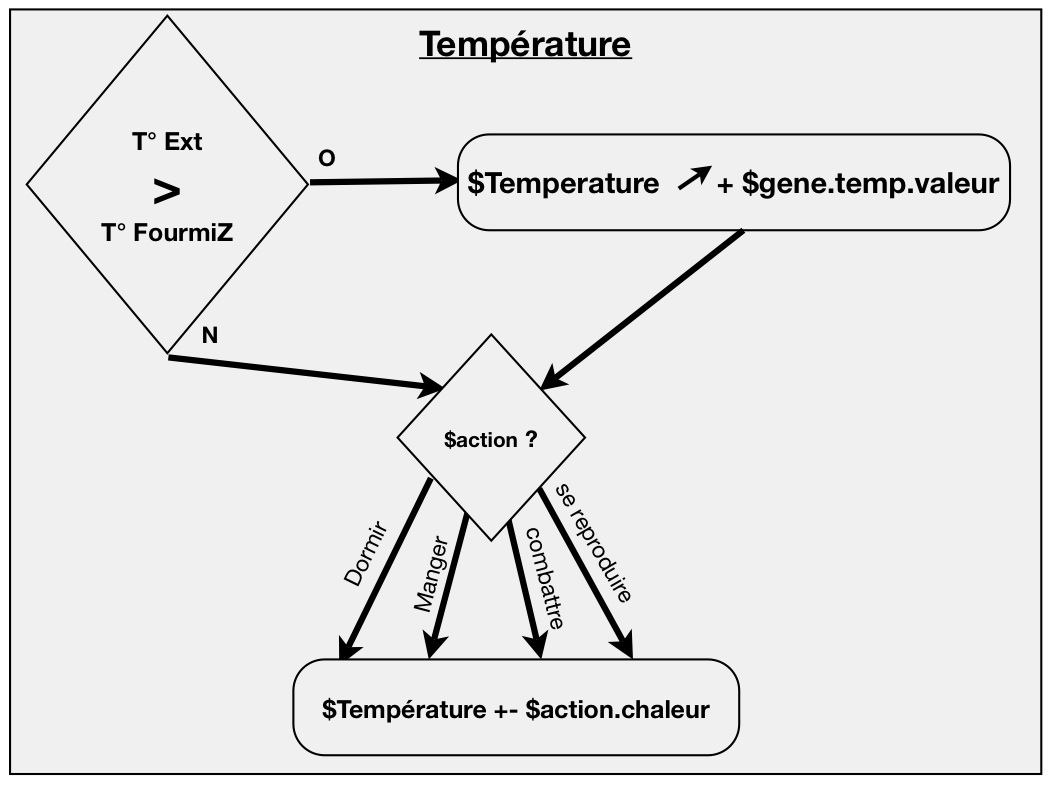
\includegraphics[width=0.5\linewidth]{images/cortex01.jpg}
	\end{center}
		
	\item Dépense l'eau en fonction de l'action de la \CoCiX.(voir \ref{hydro} page \pageref{hydro})\\
	\begin{center}
		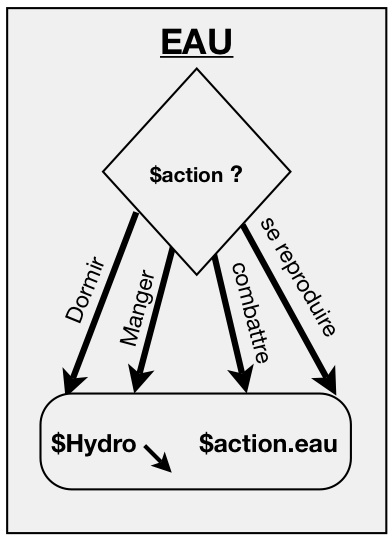
\includegraphics[width=0.5\linewidth]{images/cortex02.jpg}
	\end{center}
		
	\item Dépense les calories en fonction de l'action de la \CoCiX.(voir \ref{depense_calorique} page \pageref{depense_calorique})\\
	\begin{center}
		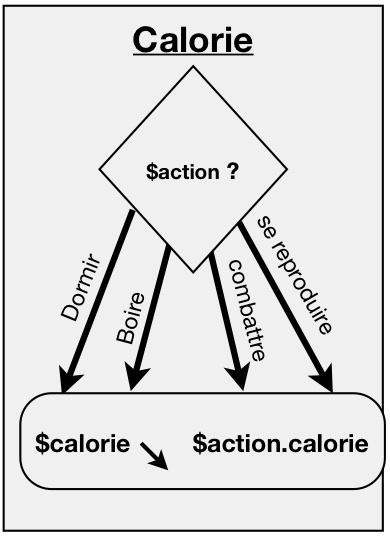
\includegraphics[width=0.5\linewidth]{images/cortex03.jpg}
	\end{center}
		
	\item Calcul les \textit{variations} de santé de la \CoCiX.(voir \ref{sante} page \pageref{sante})\\
	\begin{center}
		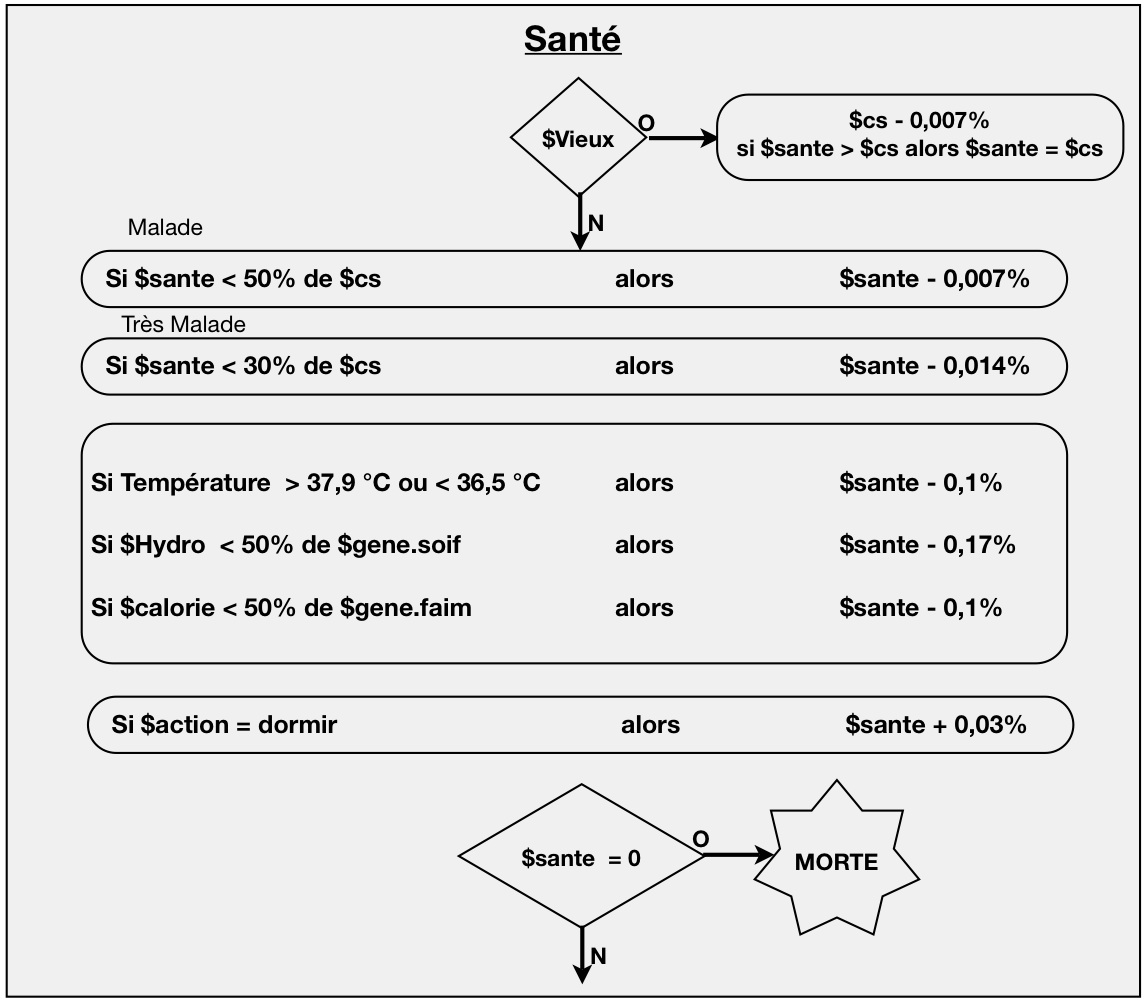
\includegraphics[width=1\linewidth]{images/cortex04.jpg}
	\end{center}
	
	\item Met à Jour les \textit{balises d'alerte}.
	\begin{center}
		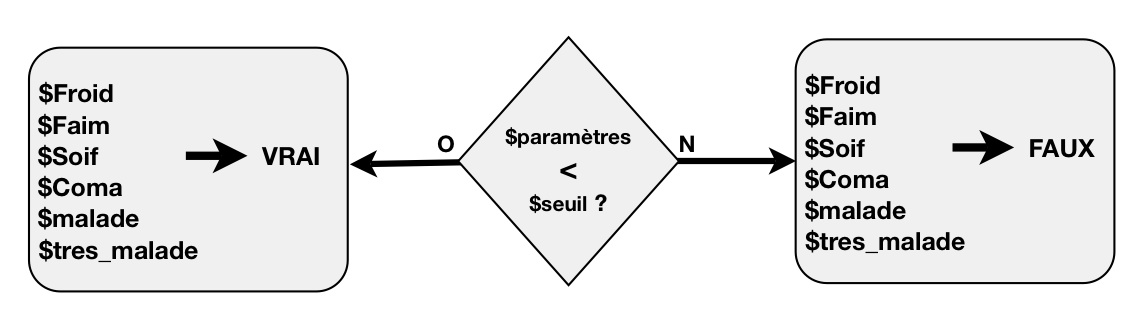
\includegraphics[width=1\linewidth]{images/cortex05}
	\end{center}

	\item Récupère le marqueur \textbf{cycle\_journalier} (voir chap \ref{jour_nuit} page \pageref{jour_nuit})\\
	
	\item Met à jour le paramètre \textbf{desire} en fonction de tous ces paramètres calculés.\\

\end{enumerate}
L'ordre de décision est capital car c'est ici que va se jouer les actions futures de la \CoCiX : \\

\subsection{Désires}\label{desire}
\subsubsection{généralités}
Les désires sont indiqués par le paramètre \textbf{desire}. Il est \textit{mise à jour} par le \textit{Cortex d'Etat} (Voir chap \ref{cortex_etat}).\\
Il matérialise les besoins vitaux des \CoCiX.\\

\subsubsection{Les désires}
Voici la liste des \textit{Désires} possibles (verbes à l'infinitif) : \\
\begin{itemize}
	\item \textit{Agresser}
	\item \textit{Boire}
	\item \textit{Dormir}
	\item \textit{Deposer}
	\item \textit{Manger}
	\item \textit{Pondre}
	\item \textit{Se\_chauffer}
	\item \textit{Se\_soigner}
	\item \textit{Recolter}
	\item \textit{Se\_reproduire}\\
\end{itemize}

\begin{center}
	\underline{Ordre des décisions du \textbf{\$desire} : }
\end{center}
S'il fait jour (\textbf{jour\_nuit() == JOUR}) :\\
\begin{enumerate}
	\item Si \textbf{coma} est à \textbf{VRAI}, \textbf{desire} = \textit{Dormir} et \textbf{action} = \textit{Dort}.
	\item Si \textbf{tres\_malade} est à \textbf{VRAI}, \textbf{desire} = \textit{Se\_soigner}.
	\item Si \textbf{Fecondee} est à \textbf{VRAI}, \textbf{desire} = \textit{Pondre}.
	\item Si \textbf{soif} est à \textbf{VRAI}, \textbf{desire} = \textit{Boire}.
	\item Si \textbf{malade} est à \textbf{VRAI}, \textbf{desire} = \textit{Se\_soigner}.
	\item Si \textbf{faim} est à \textbf{VRAI}, \textbf{desire} = \textit{Manger}.
	\item Si \textbf{froid} est à \textbf{VRAI}, \textbf{desire} = \textit{Se\_chauffer}.
\end{enumerate}

S'il n'y a aucune Balise d'alerte alors la \CoCiX pourra avoir envie de : \\
\begin{itemize}
	\item se reproduire si son cycle sexuel le permet : 
	\textbf{desire}= \textit{Se\_reproduire} \\
	\item d'agresser si elle est agressive : 
	\textbf{desire}= \textit{Agresser} \\
	\item de récolter pour les femelles qui ne se reproduisent pas : 
	\textbf{desire}= \textit{Recolter} !!\\
	\item de dormir si aucune option n'est possible:
	\textbf{desire}= \textit{Dormir} \\
\end{itemize}
Si non :\\

1. Si \textbf{jour\_nuit() == CREPUSCULE}  Alors \textbf{desire}  = Dormir, s'il n' y a aucune Balise d'alerte (faim, froid etc...)\\
Première heure de la nuit.\\

2. Si \textbf{jour\_nuit() == NUIT}  Alors \textbf{action}  = Dort.\\

Une fois le paramètre \textbf{desire} positionné, c'est le \textit{Cortex d'action} qui prend le relais pour définir l'action de la \CoCiX (voir \ref{cortex_action}).\\

\subsubsection{Structure de l'\textit{Objet} desire}
Le nom de l'\textit{Objet} \textbf{desire} est un verbe à l'\underline{infinitif}. Sa structure interne de l'\textit{Objet} \textbf{desire} est :\\
\begin{itemize}
	\item \textit{Objet} \textbf{Action}.
	\item \textit{Objet} \textbf{Alternative}.
	\item \textit{Methode} \textbf{Fonction\_Valide}.\\
\end{itemize}

\underline{\textit{Objet} \textbf{Action}}

L'\textit{Objet} \textbf{Action} est un \textit{Objet} gérant l'action permettant d'assouvir le désire (\textbf{desire}) de la \CoCiX.\\

\underline{\textit{Objet} \textbf{Alternative}}
L'\textit{Objet} \textbf{Alternative} est un \textit{Objet} indiquant quelle action peut être entreprise si l'action (\textbf{Action}) n'est pas possible.\\

\underline{\textit{Methode} \textbf{Fonction\_Valide}}
La \textit{Méthode} \textbf{Fonction\_Valide} est une \textit{Méthode} indiquant si l'Action est faisable ou non.\\

\underline{Liste des \textit{Objets} \textbf{Desire}}
\begin{lstlisting}
Manger:
	Manger.Action = Mange;
	Manger.Alternative = Cherche_Manger;
	Manger.Fonction_Valide = peut_manger();
Boire:
	Boire.Action = Boit;
	Boire.Alternative = Cherche_Eau;
	Boire.Fonction_Valide = peut_boire();
Se_Reproduire:
	Se_Reproduire.Action = Reproduit;
	Se.Reproduire.Alternative = Cherche_Partenaire;
	Se_Reproduire.Fonction_Valide = peut_se_reproduire();
Dormir:
	Dormir.Action = Dort;
	Dormir.Alternative = Rentre;
	Dormir.Fonction_Valide = peut_dormir();
Se_Soigner:	
	Se_Soigner.Action = Se_Soigne;
	Se_Soigner.Alternative = Rentre;
	Se_Soigner.Fonction_Valide = peut_se_soigner();
Se_Chauffer:	
	Se_Chauffer.Action = Rentre;
	Se_Chauffer.Alternative = Rentre;
	Se_Chauffer.Fonction_Valide = peut_se_rechauffer();
Pondre:	
	Pondre.Action = Pond;
	Pondre.Alternative = Rentre;
	Pondre.Fonction_Valide = peut_pondre();
Recolter:	
	Recolter.Action = Recolte;
	Recolter.Alternative = Cherche_Recolter;
	Recolter.Fonction_Valide = peu_recolter();
Deposer:	
	Deposer.Action = Depose;
	Deposer.Alternative = Rentre;
	Deposer.Fonction_Valide = peut_deposer();
Agresser:	
	Agresser.Action = Agresse;
	Agresser.Alternative = Cherche_Noise;
	Agresser.Fonction_Valide = peut_agresser();		
\end{lstlisting}	


\newpage

\subsection{Le Cortex d'Action}\label{cortex_action}

Le \textit{Cortex d'Action} représente la partie "consciente" de la \CoCiX.\\
Le \textit{Cortex d'Action} va déterminer l'action que la \CoCiX va pouvoir faire, en tenant compte de ses désires (\textbf{desire}), déterminés par le \textit{Cortex d'Etat} (Voir chap \ref{cortex_etat} page \pageref{cortex_etat}) et de ses possibilités (terrain, partenaire, lieu etc...).\\

Le Cortex d'action est un programme autonome lié à chaque \CoCiX et déclenché par cron.\\

\begin{center}
	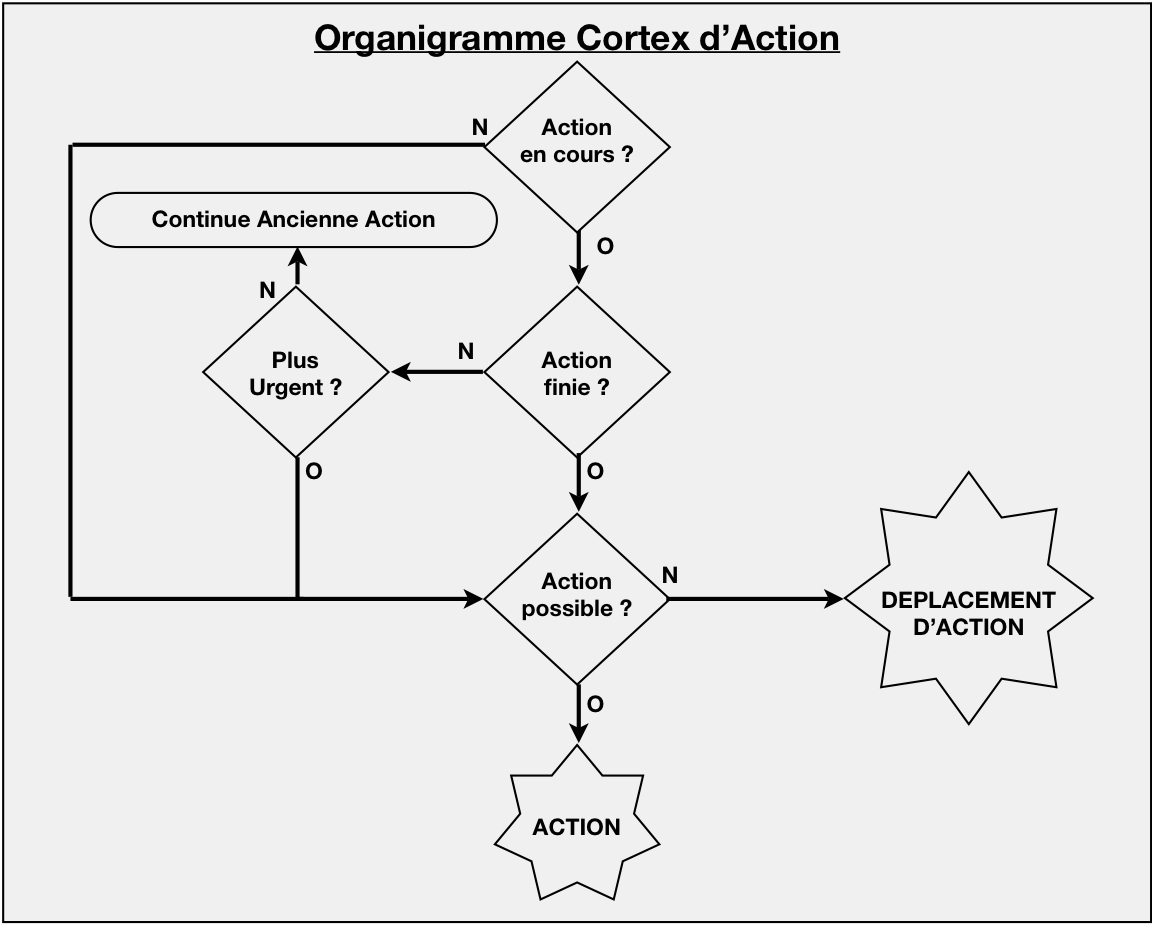
\includegraphics[width=0.8\linewidth]{images/cortex_action.jpg}
\end{center}

Pour fonctionner, le \textit{Cortex d'Action} va récupérer le paramètre \textit{Objet}  \textbf{Desire} transmis par le \textit{Cortex d'Etat} ( Voir \ref{cortex_etat} page \pageref{cortex_etat}).\\

\textit{exemple} : \\
\begin{quote}
	
	Le \textit{Cortex d'Etat} renvoie un paramètre \textbf{Desire} = Boire : \\
	
	\begin{itemize}
		\item \textbf{Desire}.Action = Boit;
		\item \textbf{Desire}.Alternative = Cherche\_Eau;
		\item \textbf{Desire}.Fonction\_Valide = \textit{peut\_boire()}.\\
	\end{itemize}
	
\end{quote}
Le Cortex d'Action utilise des paramètres variables permettant de contrôler l'état de l'action:
\textbf{temps\_action} de sa partenaire.\\
Le paramètre d'état  
\begin{itemize}
	\item \textbf{temps\_action} : indique depuis combien de temps l'action se fait (en minute)
	\item \textbf{Partenaire} : Partenaire si l'action implique une autre \CoCiX \textit{(Soins, reproduction, combat etc\dots)}
\end{itemize}
\section{Les Actions}\label{action}
\subsection{Principe}
\textbf{Action} est en fait un \textit{Objet} marquant l'action que fait la \CoCiX.\\

\subsection{Structures de l'Objet Action}
Les Actions ont les \textit{attributs} suivants:
\begin{itemize}
	\item \textbf{.id\_action} : Numéro d'identification unique (lié éventuellement à une table)
	\item \textbf{.action} : Verbe conjugué correspondant à l'action effectuée.
	\item \textbf{.chaleur} : Correspond à la variation de température qu'induit l'action  (en \degres C par minute).
	\item \textbf{.eau}  : Correspond à la quantité d'eau dépensée en $\mu$L par minute.
	\item \textbf{.calorie} : Correspond aux nombres de calories dépensées par minute pour l'action.
	\item \textbf{.duree} : Correspond au nombre de minutes qu'il faut pour exécuter cette action.
	% % %\item .\textbf{temps} : indique le temps depuis combien de temps l'action se fait (en minute).
	\item \textbf{.deplacement} : Booléen indiquant si cette action est un déplacement.
	\item \textbf{.termine} : Booléen indiquant si cette action est terminée.
	\item \textbf{.fonction} : Nom de la fonction executant l'action.
	\item \textbf{.peut\_arreter} : Booléen indiquant si l'action peut-être arrêter.\\
\end{itemize}
Les Actions ont les \textit{Méthodes} suivants:
\begin{itemize}
	\item \textbf{.go()} : Exécute l'action.
\end{itemize}
\subsection{Liste des Actions (Verbes conjugués)}

	\begin{center}
		\begin{tabular}{ll}
			\textit{Agresse} &\textit{Fuit}\\ 
			\textit{Boit}&\textit{Mange}\\ 
			\textit{Cherche\_eau}&\textit{Pond}\\ 
			\textit{Cherche\_manger}&\textit{Rechauffe}\\ 
			\textit{Cherche\_partenaire}&\textit{Recolte}\\ 
			\textit{Combat}&\textit{Rentre}\\ 
			\textit{Depose}&\textit{Reproduit}\\ 
			\textit{Dors}&\textit{Soigne}\\ 
		\end{tabular}\\

\begin{tabular}{|p{0,5cm} | p{4cm} |p{2,5cm} | p{1,5cm}|p{0,5cm}|p{0,8cm}|p{1cm}|p{1cm} |} \hline
\rowcolor{red} id & \textbf{action}  & \textbf{desire} & \textbf{chaleur} & \textbf{eau} & \textbf{cal} & \textbf{durée} & \textbf{dep}\\ \hline
% id		non     desire           chaleur      eau    calorie  durée  depla  
			1&Boit & Boire & - & 0 & 0,3 & - & non\\ \hline
			2&Cherche\_eau & Boire & 0,02\degres C  & 1 & 1 & - & oui\\ \hline
			3&Cherche\_manger & Manger & 0,02\degres C  & 1 & 1 & - & oui\\ \hline
			4&Cherche\_partenaire & Se\_reproduire & 0,02\degres C  & 1 & 1 & - & oui\\ \hline
			5&Combat & - & 0,1\degres C & 3 & 2 & - & non\\ \hline
			6&Dort & Dormir &-0,05\degres C &0,01 & 0,016 & - & non\\ \hline
			7&Fuit & - & 0,1\degres C & 3 & 1,5 & 3 & oui\\ \hline
			8&Mange & Manger & -0,05\degres C & 0,5 & 0,5 & 5 & non\\ \hline
			9&Pond & Pondre & 0,1\degres C & 3 & 3 & 5 & non\\ \hline
			10&Rechauffe & Se\_rechauffer & - & 1 & 3 & - & non\\ \hline
			11&Rentre & Se\_soigner ou Se\_rechauffer & 0,01\degres C & 1 & 1 & - & oui\\ \hline
			12&Reproduit & Se\_reproduire & 0,1\degres C & 3 & 1,8 & 5 & non\\ \hline
			13&Soigne & - & 0,05\degres C & 3 & 3 & 10 & non\\ \hline
			14&Se\_soigne &Se\_soigner & 0,02\degres C & 0,1 & 1 & 5 & non\\ \hline
			15&Recolte & Recolter & 0,05\degres C & 1 & 1 & 3 & non\\ \hline
			16&Depose & Deposer & 0,02\degres C & 1&1&1&non\\ \hline
			17&Cherche\_recolter & Recolter & 0,02\degres C & 1 & 1 & - & oui\\ \hline
			18&Agresse&Agresser&0,3\degres C &5&2&5&non\\ \hline
			19&Cherche\_noise&Agresser&0,03\degres C &1&1&-&oui\\ \hline
			
		\end{tabular}
	\end{center}

\newpage	
\chapter{Le Génome}\label{genome}
\section{Principes et Généralités}
Le génome est une base de donnée contenant tous les gènes possibles des \CoCiX.
Il sert au moment de la procréation, à initialiser tous les gènes de la nouvelle \CoCiX.\\

Un gène est un \textit{Objet} composé d'attributs :

\begin{itemize}
	\item \underline{Un nom}  : \textit{Taux\_Fecondite} , \textit{Agressivité} etc...\\
	\item \underline{Un Identifiant unique} : \textbf{(ID)}  Numéro donnée par la base de donnée.\\
	\item \underline{L'Influant} \textbf{(influant)} : Si le gène est influent  \textbf{influent} donne le nom du paramètre d'état. Il est vide si le gène n'est pas influent (voir  \ref{genetique} page \pageref{genetique}).\\
	\item \underline{Un code de transmission} \textbf{(transmission)} :\\
	Ce code peut prendre comme valeur :
	\begin{itemize}
		\item P : Transmission par le père
		\item M : Transmission par la mère
		\item PM : Transmission par le père OU la Mère.
		\item pm : Transmission de Père en fils ou de Mère en fille.
		\item GP : Transmission par un des 2 Grand-pères (Saute une génération).
		\item GM : Transmission par une des 2  Grand-mères (Saute une génération).
		\item H : Transmission par les Hommes (Père, et les 2 grand-pères).
		\item F : Transmission par les Femmes (Mère et les deux grand-mères).
		\item 6p: Transmission par les 6 membres (Père, Mère, 2 grand-pères et 2 grand-mères).
	\end{itemize}
	
	\begin{quote}
		\textit{Exemples : }
		\textit{L'agressivité} est un gène codé \textbf{H}, c'est à dire qu' à la procréation, l'ordinateur choisira au hasard, entre les paramètres d'agressivité (\textit{\$gene.agressivite.taux}) du Père et des deux grand-pères, et l'affectera à l’œuf.\\
		
		Le \textit{taux de fécondation} est un paramètre influencé par le gène Fécondation codé \textbf{M}, donc à la procréation, l'ordinateur affectera le même gène que la mère à sa fille.\\		
	\end{quote}
\end{itemize}
\section{Table du Genome}\label{liste_gene}
\begin{center}
\begin{tabular}{|l|c|c|l|}\hline
\rowcolor{green}\textbf{nom}  & \textbf{Influant} & \textbf{\small{Transmission}} & \textbf{Ref}\\ \hline

.agressivite & \% & H & page \pageref{agressivite} \\ \hline
.assimilation\_calorique & \$calories & 6p & page \pageref{nourrir} \\ \hline
.assimilation\_hydrique & \% & 6p & page \pageref{hydro} \\ \hline
.calorie & \$cc  & PM & page \pageref{cc} \\ \hline
.faim  & \$calories & 6p & page \pageref{faim} \\ \hline
.froid & \$temperature & H & page \pageref{froid} \\ \hline
.hydro & \$hydro & GP & page \pageref{hydro} \\ \hline
.recolte & \$recolte & F & page \pageref{param_action}\\ \hline
.recup\_sommeil & \$sante & M & page \pageref{sante}\\ \hline
.sante  & \$sante & H &  page \pageref{sante}\\ \hline
.satiete & \% & 6p & page \pageref{nourrir}\\ \hline
.seuil\_malade & \% & 6p & page \pageref{sante}\\ \hline
.seuil\_tres\_malade & \% & 6p & page \pageref{sante}\\ \hline
.soif & \% & GP & page \pageref{soif} \\ \hline
.soins & \% & GM & page \pageref{repos} \\ \hline
.souffre\_faim & \% & 6p & page \pageref{faim} \\ \hline
.souffre\_soif & \% & 6p & page \pageref{soif} \\ \hline
.temp & \$temperature & PM & page \pageref{temperature} \\ \hline
.vieux & \$vieux & PM & page \pageref{vieillesse} \\ \hline
.vivacite & \$vivacite & GM & page \pageref{vivacite} \\ \hline
\end{tabular}
\end{center}
\chapter{Sexualité \& Reproduction}\label{sexualite}
\section{Principes \& généralités}

Lorsque deux \CoCiX de sexe différents sont sur la même case, que le mâle est actif sexuellement et la femelle disponible et fécondable, le processus de reproduction peut commencer.\\
Une des \CoCiX peut "entreprendre" l'autre en informant son \textbf{Cortex d'Action} (voir \ref{cortex_action} page \pageref{cortex_action}). Les deux \CoCiX vont alors copuler.\\
A la fin de la reproduction, les gènes du père et de la mère, vont former une \CoCiX "virtuelle" avec comme lien un numéro \textbf{Id\textit{}} (voir \ref{identite} page \pageref{identite}).\\
Ce numéro id est affecté à la mère qui devient fécondée.\\
Lorsque la \CoCiX fécondée passe dans son cycle de ponte (voir \ref{cycle_sexuel} page \pageref{cycle_sexuel}), elle déposera l’œuf sur la case où elle se trouve. Cet œuf aura alors comme case de naissance cet endroit.\\

\section{Quand la reproduction est-elle possible ?}

Pour qu'il puisse y avoir reproduction, il faut  : que deux \CoCiX de sexe différents soient sur la même case, que les deux soient matures et disponibles, et enfin que l'un des deux en exprime le désire !!\\

l'action \textbf{Reproduit} est subordonnée au désire \textbf{Se\_Reproduire} (voir \ref{cortex_action} page \pageref{cortex_action}). Il a comme fonction de validation : \textit{peut\_se\_reproduire()} \\


\begin{lstlisting}[frame = single,caption={peut\_se\_reproduire()en PHP TODO}]
private function peut_se_reproduire($debug = false) {
$Partenaire = partenaire($this->case,$this,$debug);
return($Partenaire); 
}
\end{lstlisting}
La fonction \textbf{\textit{partenaire(\$this->case,\$this,\$debug)} }renvoie le numéro d'un partenaire potentiel pour la \CoCiX placée sur la case \textit{\textbf{case}} ou 0 s'il n'y en a pas.\\

S'il n'y a pas de partenaire, l'action \textbf{Reproduit} est subordonnée à \textit{l'action alternative}  \textbf{Chercher\_Partenaire} (voir \ref{cortex_action} page \pageref{cortex_action}), qui ne fait que regarder autour de la \CoCiX s'il y a des partenaires potentiels, se déplacer vers eux ou bouger pour en trouver. Cette Fonction doit être une méthode implémentée dans l’Environnement.(Voir Chap\ref{carte_monde} p \pageref{carte_monde})\\

\section{La reproduction}
Lorsque tout est en place, les deux \CoCiX vont pouvoir se reproduire.\\
La \textit{Méthode} \textbf{.go()} va alors être déclenchée au niveau du \textit{Cortex d'Action}, par l'une des \CoCiX en question, qui en informera l'autre. La copulation a une durée d'environ 5mn et c'est le mâle qui informe la femelle du temps qu'il va mettre en mettant à jour la variable .\textbf{temps\_action} de sa partenaire.\\
Le paramètre d'état \textbf{Partenaire} est renseigné pour chaque \CoCiX.(voir \ref{fecondee} page \pageref{fecondee})\\

\section{Un ou une Nouveau(ele) \CoCiX}
\subsection{principe}
Lorsque la copulation est terminée, la femelle enclenche la fonction \textit{reproduction()}qui engendrera la plupart des paramètres de la nouvelle \CoCiX. La fonction renvoie un numéro \textbf{Id} de la nouvelle \CoCiX, qui va être rentrée dans le paramètre \textbf{id\_oeuf} de la mère.\\

\subsection{Fonction \textit{reproduction()}}
Cette fonction est de la forme \textbf{reproduction(Pere,Mere)} avec \textbf{Pere} \textit{l'Objet} \CoCiX du père et \textbf{Mere}  \textit{l'Objet} \CoCiX de la mère.\\
La fonction contient plusieurs étapes :

\begin{itemize}
	\item \textit{\underline{Insertion}} dans la base de donnée  d'une nouvelle \CoCiX. On lui met la plupart des paramètres à 0 sauf celui des identifiants des parents : (\textbf{.idpere} et \textbf{.idmere}). On récupère alors le numéro id de cette nouvelle \CoCiX, afin de rentrer dans la table gènes, le patrimoine génétique de l’œuf.\\
	
	\item \textit{"\underline{Mixagénèse}"} de la nouvelle \CoCiX : \\
	Cette étapes consiste à prendre les gènes, un par un dans la table du génome (voir \ref{genome} page \pageref{genome}), puis à leur appliquer: \\ 
	
	\begin{enumerate}
		
		\item \underline{Transmission génétique} : cette étape récupère les gènes de chaque parents et les copies dans le patrimoine de l'oeuf : \\
		\begin{verbatim}
		Genes[nom du gène].pere = Pere.Genes[nom du gène].valeur
		Genes[nom du gène].mere = Mere.Genes[nom du gène].valeur
		Genes[nom du gène].gp_mere = Mere.Genes[nom du gène].pere
		Genes[nom du gène].gp_pere = Pere.Genes[nom du gène].pere
		Genes[nom du gène].gm_mere = Mere.Genes[nom du gène].mere
		Genes[nom du gène].gm_pere = Pere.Genes[nom du gène].mere
		
		\end{verbatim}
		
		\item Chaque gène donne son mode de transmission et l'on choisit au hasard entre les gènes transmis, la valeur à attribuer au gène de l’œuf.\\
		
		\begin{quote}
			\underline{exemple : }
			pour le gène \underline{\textbf{.soif}}, transmit par GP, on va prendre au hasard la valeur du gène \underline{\textbf{.soif}} des deux grand-peres de l’œuf, c'est à dire entre : \\
			Genes['soif'].gp\_mere et\\
			Genes['soif'].gp\_pere\\
			
			Le hasard de notre exemple veut que cela soit celui du grand-père maternelle ...\\
			On initialise donc la valeur de ce gène avec la valeur du grand-père maternelle : \\
			
			\textbf{Genes['soif'].valeur} = Genes['soif'].gp\_mere\\
			
		\end{quote}
		\item \underline{Modification "\textit{consanguine}" } : Tous les gènes subissent une altération dûe à la consanguinité. Le paramètre renvoyé par la fonction \textit{degre(\textbf{CoCiX},\textbf{CoCiX})} est un pourcentage d'altération  de + ou - cette valeur.\\
		
		\item \underline{Mutation environnementale} : Le facteur environnemental est tributaire du taux de radioactivité de la case où à eu lieu la copulation. La valeur du gène est affecté de +ou - 10\% de la radioactivité.\\
		
		A noter que les modifications sont cumulées pour le calcul final de la valeur du gène :\\
		\begin{quote}
			\underline{exemple : }
			La valeur du gène \underline{\textbf{.soif}} avant les modificateurs est de 60\%. La fécondation a eu lieu sur une case ayant un taux de radioactivité = 40 Rad, on a alors :\\
			\begin{itemize}
				\item + ou -5\% de modification naturelle\\
				\item 10\% de 40 =  + ou -4\% de Mutation environnementale\\
			\end{itemize}
			On a en tout 9\% en plus ou en moins de modification de la valeur du Gène \textbf{\underline{.soif}}, soit une valeur comprise entre \textbf{54,6\% }et \textbf{65,5\%} .\\
			
		\end{quote}
		\item Récupération des valeurs importantes, affectant des \textit{Paramètres d’État} (voir \ref{param_etat} page \pageref{param_etat}) ou génétiques (voir \ref{genetique} page \pageref{genetique}) : \\
		\begin{itemize} 
			\item {\textbf{.vieux}} : initialisé par le gène : \textbf{Genes['vieux']}. (voir \ref{vieillesse} page \pageref{vieillesse})
			\item {\textbf{.ch}} : Le \textbf{C}apital \textbf{H}ydrique est initialisés par le gène \textbf{Genes['hydro']}.(voir \ref{hydro} page \pageref{hydro})
			\item {\textbf{.cc}} : Le \textbf{C}apital \textbf{C}alorique est initialisé par le gène \textbf{Genes['calorie']}.(voir \ref{alimentation} page \pageref{alimentation})
			\item {\textbf{.cs}} :  Le \textbf{C}apital \textbf{S}anté est initialisé par le gène \textbf{Genes['sante']}.(voir \ref{sante} page \pageref{sante})
		\end{itemize}
		\item \underline{Enregistrement} du gène de l’œuf dans la base de donnée \textit{Gènes}:\\
		Chaque gènes ainsi crées à partir du patrimoine génétique de la mère et du père, est enregistré dans la base de données \textit{Gènes} associé au numéro de la future \CoCiX.\\
		
	\end{enumerate}
	\item On a récupéré avec la \textit{Mixagénèse}, les paramètres états et génétiques (\textbf{.vieux}, \textbf{.ch}, \textbf{.cc} et \textbf{.cs}) qui nous permettent de mettre à jour la future \CoCiX.  Les paramètres \textbf{.case} et \textbf{.date\_naissance} sont laissés à 0 tant que l’œuf n'a pas été pondu.\\
	\item La fonction retourne enfin le numéro de l’œuf à la mère.\\
	
\end{itemize} 

\section{La ponte}\label{ponte}
À la période de ponte la femelle va avoir le \textit{désire} de pondre au niveau de son \textit{Cortex d'Etat} : \\
\begin{quote}
	\textbf{.Desire} = \textbf{Pondre}\\
\end{quote}

L'action \textbf{Pond} est subordonnée au désire de Pondre et à une fonction de validation : \textit{peut\_pondre}().\\

La \CoCiX peut pondre si : 
\begin{itemize}
	\item C'est une femelle.
	\item Elle est fécondée.
	\item C'est son cycle de ponte.
	\item Une place est libre sur la case.\\
\end{itemize}

\newpage
\chapter{Les Combats}\label{combat}
\section{Principe}

Les \CoCiX ont un gène d'agressivité (voir page \pageref{agressivite}) , et peuvent avoir le désire de combattre et de chercher des ennemis potentiels auprès de ses congénères adultes et de même sexe.\\
Le principe est assez similaire à la reproduction (voir chap \ref{sexualite} p \pageref{sexualite}). \\

Une des \CoCiX peut attaquer l'autre en informant son \textbf{Cortex d'Action} (voir \ref{cortex_action} page \pageref{cortex_action}). Les deux \CoCiX vont alors combattre.\\

\section{Quand le combat est-elle possible ?}

Pour qu'il puisse y avoir combat, il faut  : qu'une  \CoCiX agresse une autre \CoCiX du même sexe sur la même case.\\

l'action \textbf{Agresse} est subordonnée au désire \textbf{Agresser} (voir \ref{cortex_action} page \pageref{cortex_action}). Il a comme fonction de \textit{validation} : \textbf{peut\_agresser()}. \\

S'il n'y a pas de \CoCiX à agresser, l'action AGRESSE est subordonnée à \textit{l'action alternative} \textbf{Chercher\_Noise()} (voir \ref{cortex_action} page \pageref{cortex_action}), qui ne fait que regarder autour de la \CoCiX s'il y a des ennemis potentiels, se déplacer vers eux ou bouger pour en trouver.\\

\section{Le Combat}
Lorsque le combat commence, c'est la \CoCiX qui a son \textbf{.id} le plus petit qui compte les tours.\\
les \textit{actions} se déroulent dans un ordre précis : \\

\begin{enumerate}
	\item Initiative. (qui attaque en premier)
	\item début du tour attaquant.
	\item jet du dé d'attaque
	\item jet du dé de défense
	\item rapport force endurance
	\item rapport de blessures
	\item rapport de courage pour savoir si la \CoCiX fuit.
	\item fin du tour attaquant, début tour défenseur.
	\item seq 3-6\\
\end{enumerate}

{\large TODO: Détailler les combats dans l'esprit \textit{Warhammer} !}

%%%%%%%%%%%%%%%%%%%%%%%%%%%%%%%%%%%%%%%%%%%%%%%%%%%%%%%%%
%  E N V I R O N N E M E N T  					  		%
%%%%%%%%%%%%%%%%%%%%%%%%%%%%%%%%%%%%%%%%%%%%%%%%%%%%%%%%%

\newpage
\part{Environnement}\label{environnement}
%%% GENERALITE %%%
\chapter{Généralité, notion de temps et bases de données}\label{jour_nuit}

L'environnement des \CoCiX est un véritable petit \textit{Monde} dans lequel, elles vont pouvoir, se déplacer, puiser des ressources (nourriture, eau etc...), faire des rencontres ! se reproduire etc...\\
Ce monde est autonome, c'est à dire qu'un programme, va le fait évoluer, tant en ressource, qu'en météo etc...\\

Il a sont propre temps, gérer par des \textit{crons}\footnotemark[1] du serveurs.\\
Plusieurs bases de données vont être nécessaires pour représenter l'environnement : \\
\begin{itemize}
	\item Une base de donnée pour les \textit{cases} du monde (voir \ref{bd_monde} ).
	\item Une base de donnée des cycles (Jour-Nuit, Jours).\\
\end{itemize}

\section{La Base Cycles}\label{base_cycles}
La base de donnée \textit{cycles} contient plusieurs marqueurs : 
\begin{enumerate}
	\item  \textbf{\$bigbang},indique la date de la création du monde.
	\item  \textbf{\$vitesse},indique la vitesse à laquelle passe le temps.
	\item  \textbf{\$minute} est incrémenté chaque minute par \textit{crons}\footnotemark[1]. Il augmente de 1 multiplié par le marqueur  \textbf{\$vitesse}. (exemple : si \textbf{\$vitesse} = 4, chaque minute serveur augmente le temps du monde de 4 minutes).
	\item  \textbf{\$heure} : indique l'heure du monde.
	\item \textbf{\$ jour\_nuit} est un entier = JOUR, NUIT ou CREPUSCULE (constantes)
	\item \textbf{\$jours} indique le jour du monde. C'est aussi le nombre de jour écoulés depuis le Bigbang !
	\item \textbf{\$heure\_nuit} donne l'heure où il fait nuit.
	\item \textbf{\$heure\_jour} donne l'heure où il fait jour
\end{enumerate}
Cette base de données est automatiquement mise à jour par \textit{cron}\footnotemark[1] de serveur.\\

\footnotetext[1]{\textit{cron} est le nom d'un programme qui permet aux utilisateurs des systèmes Unix d'exécuter automatiquement des scripts, des commandes ou des logiciels à une date et une heure spécifiées à l'avance, ou selon un cycle défini à l'avance.}

\begin{lstlisting}[caption={jour\_nuit\_cron\_php}]
%\begin{verbatim}
//Cycle JOUR-NUIT
// par le cron
include_once("connexion.php");

define("JOUR",1);
define("NUIT",-1);
define("CREPUSCULE",0);

$sql1 = "SELECT * FROM cycles";

$resulta_requete = mysql_query($sql1);
if($resulta_requete <> false) {
$cycles = mysql_fetch_object($resulta_requete);

$vitesse = $cycles->vitesse;
$minute = $cycles->minute;
$heure = $cycles->heure;
$jours = $cycles->jours;

$heure_jour = $cycles->heure_jour;
$heure_nuit = $cycles->heure_nuit;
$jour_nuit = $cycles->jour_nuit;

// incremente le cycle journalier
$minute = $minute + ($vitesse);
if($minute >= 60) {

// une heure de passee
$minute = ($minute-60);
$heure++;
if($heure >= 24) {
// un jour de passe
$heure = $heure-24;
$jours++;
}
} 
// determination de la luminosite : 

if(($heure == ($heure_nuit - 2)) or ($heure == ($heure_nuit-1))) {
$jour_nuit = CREPUSCULE; // Il faut aller se coucher
} else {

if($heure >= ($heure_nuit) or $heure < $heure_jour) {

// il fait nuit
$jour_nuit = NUIT;
} else {
// il fait jour
$jour_nuit = JOUR;
}
}

echo "Jour # $jours , $heure h, $minute mn</br>";
switch($jour_nuit) {
case -1:
echo "Il fait nuit.";
break;
case 0:
echo "Il va bientot faire nuit.";
break;
case 1:
echo "Il fait jour.";
break;
}

$update = "UPDATE cycles SET minute = '".$minute."', heure = '".$heure.
"', jours = '".$jours."', jour_nuit = '".$jour_nuit."' ,date = NOW( ) WHERE id=1";

mysql_query($update);

mysql_close($liendb);

} else {
die("Impossible de charger les cycles sur le serveur...");
return false;
}

%\end{verbatim}
\end{lstlisting}

\chapter{Monde}\label{carte_monde}
Le \textit{Monde} est une grille de 100 x 100 cases, dans un espace fermé.\\
Chaque case représente un espace de $1 cm^2$, pouvant contenir 2 \CoCiX maximum.

\section{Coordonnées (x,y)}\label{coordonnees}

\subsection{Principes}
Les cases sont numérotées de gauche à droite et de haut en bas.\\

Elles peuvent être aussi représentées par un couple (x,y) (x pour le nombre de cases Horizontales et y pour les Verticales).\\
La case (1,1) se situe en Haut à Gauche, et son \textbf{id} est 1.\\

Pour passer du numéro unique (\textbf{id}) au couple \textbf{(x,y)} on a :\\

x = Reste de la division entière de \textbf{id} par 100 (\textit{Modulo}). (Si le \textit{Modulo} est à 0 alors  x=100).\\

Ensuite,

\begin{equation}
y = \frac{\textbf{id} - x}{100} + 1
\end{equation}

\underline{exemple :} \\
\begin{quote}
	Notre \CoCiX TOTO est sur la case dont l'\textbf{id} est 2928.\\
	
	On a \[ x = Modulo(\frac{2928}{100}) = 28,\]
	
	et \[ y =  \frac{2928 - 28}{100} + 1  = 30.\]
	
	la case de TOTO est représentée par le couple \textbf{(28,30)}.
	
\end{quote}

\section{Orientation \& Déplacements}\label{orientation}
\subsection{Principes}
La \CoCiX devra se déplacer, et donc s'orienter.\\

Pour se déplacer :
\begin{itemize}
	\item De gauche à droite, il suffit d'ajouter 1 à son numéro unique de case.
	\item de droite à gauche, on retranche 1 au numéro unique de case.
	\item Pour monter il suffit de retrancher 100.
	\item Pour descendre d'ajouter 100.\\
\end{itemize}

L'espace étant fermé, le bord \textit{Droit} et le Bord \textit{Gauche} de la carte du monde se "\textit{touchent}", ainsi que le bord \textit{supérieur} et \textit{inférieur}.\\
Le passage du bord droit au bord gauche, se fait automatiquement par l'addition du numéro de la case.\\
De même pour le passage de gauche à droite, le retranchement  fait passer automatiquement d'un bord à l'autre.\\

Le logiciel contrôle ensuite le \textit{numéro unique} de case qui doit être compris entre 1 et 10000, en additionnant ou soustrayant 10 000. \\

\textit{\underline{Exemple}}:\\
Lorsque la \CoCiX est au bord supérieur en étant  en (10,1) soit en case n\degres 10,  Si elle monte d'une case, on retranche 100 donc sa case est  --90. En additionnant 10 000 on trouve 9910 qui est la case correspondante en bas. (10,100).\\
A l'inverse si la \CoCiX est au bord inférieur, par exemple à case 9922 (22,100), et qu'elle descend d'une case on aura 9922 + 100 = 10 022 - 10 000 = 22 case (22,1).

\subsection{Fonctions}
Voici les 4 fonctions pour se déplacer. Le paramètre passé est le numéro de la case de départ. Les fonctions renvoient la case d'arrivée après l'avoir validée : \\

\begin{lstlisting}[frame = single,caption={Fonctions de déplacements dans 'Monde'}]
fontion monte(depart){
	arrivee = depart - 100;
	retourne valide_case(arrivee);
}

fonction descend(depart){
	arrivee = depart + 100;
	retourne valide_case(arrivee);
}

fonction gauche(depart){
	arrivee = depart - 1;
	retourne valide_case(arrivee);
}

fonction droite(depart){
	arrivee = depart + 1;
	retourne valide_case(arrivee);
}
\end{lstlisting}
La fonction valide\_case() contrôle l'espace fermé : \\
\begin{lstlisting}[frame = single,caption={Fonctions dans Monde}]
fonction valide_case(case){
	Si case <= 0  retourne case+10000;
	Si case > 10000 retourne case-10000;
	Retourne case;
}
\end{lstlisting}

Nous avons ensuite les fonctions qui combinent monter, descendre, droite et gauche : \\


\begin{lstlisting}[frame = single,caption={monde.php}]
function monte_gauche($depart){
$etape = monte($depart);
$arrivee = gauche($etape);
}

function monte_droite($depart){
$etape = monte($depart);
$arrivee = droite($etape);

}

function descend_gauche($depart){
$etape = descend($depart);
$arrivee = gauche($etape);
}

function descend_droite($depart){
$etape = descend($depart);
$arrivee = droite($etape);	
}
\end{lstlisting}

\section{Base de données \textbf{Monde}}\label{bd_monde}
Le Monde des \CoCiX est représenté informatiquement par une base de donnée de 100 x 100 = 10 000 cases.
Chaque case contient des informations sous la forme de champs :\\

\begin{itemize}
	\item[\textbf{Id}] : numéro unique de la case. 
	\item[\textbf{nourriture}] : Quantité de nourriture disponible (en calories).
	\item[\textbf{humidité}] : Quantité d'eau disponible (en $\mu L$).
	\item[\textbf{temperature}] : Temperature de la case (en degré Celsius).
	\item[\textbf{CoCiX1}] : \textbf{\$id} de la première \CoCiX ( à 0 s'il n'y en a pas).
	\item[\textbf{CoCiX2}] : \textbf{\$id} de la deuxième \CoCiX ( à 0 s'il n'y en a pas).\footnote{Possibilité d'utiliser une base jumelée pour qu'il y ai autan de \CoCiX que l'on veut sur une case.}
	\item[\textbf{pheromone}] : Les \CoCiX peuvent laisser des phéromones sous la forme d'un code (TODO).
	\item[\textbf{radio}] : Taux de radioactivité en Rad.\\
\end{itemize}

\centerline{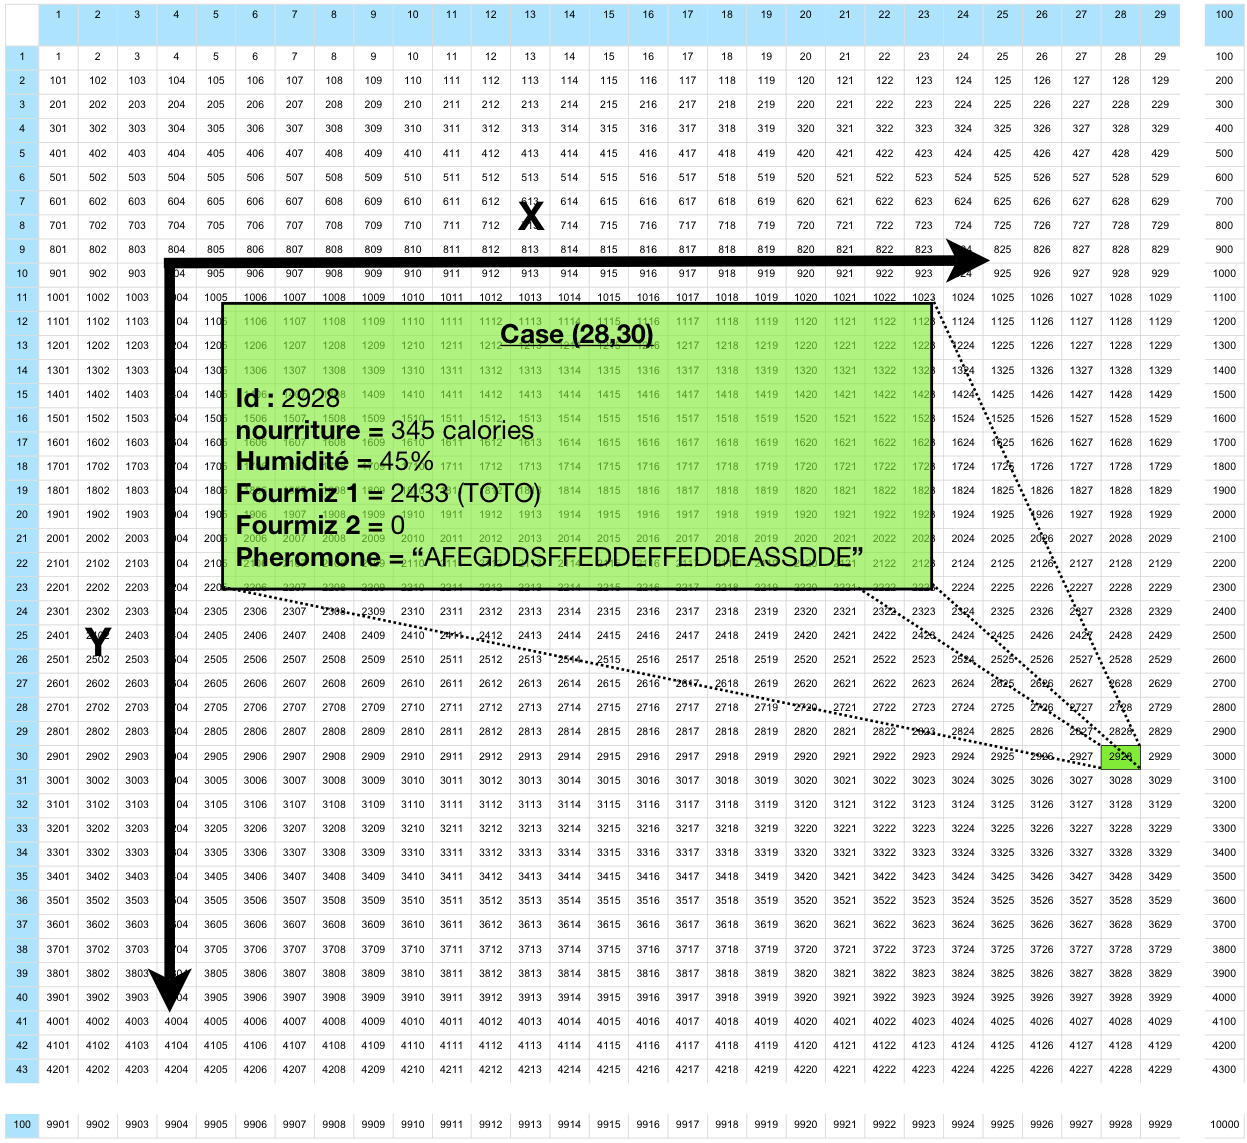
\includegraphics[width=18cm]{Monde01.png}}\label{cartemode}

\section{Fonctions}\label{methodes_monde}
Plusieurs \textit{fonctions}, appelées par la \CoCiX ou par des modules extérieurs, permettent de connaître les informations sur une case précise : \\

Ces fonctions sont pour l'instant écrite en \textit{Php}.

\subsection{Fonction Temperature()}
Cette fonction renvoi la température d'une case passée en paramètre à cette fonction : \\

\begin{lstlisting}[frame=single,caption={monde.php}]
.../...
function temperature($case) {
// renvoi la temperature exterieur de la case
if($case > 1 && $case <= 10000) {
$sql = "SELECT temperature FROM monde WHERE id='".$case."'";
$resulta_requete = mysql_query($sql);
if($resulta_requete <> false) {
$case_monde = mysql_fetch_object($resulta_requete);

return ($case_monde->temperature);

} else {
die("Impossible de charger les cycles sur le serveur...");
return 0;
}
} else die ("erreur");

}
.../...
\end{lstlisting}

%%%%%%%%%%%%%%%%%%%%%%%%%%%%%%%%%%%%%%%%%%%%%%%%%%%%%%%%%
%    								C L A S S E S             &             O B J E T S  						%
%%%%%%%%%%%%%%%%%%%%%%%%%%%%%%%%%%%%%%%%%%%%%%%%%%%%%%%%%

\newpage
\part{Classes et Objet} \label{classes}
\chapter{Les déclarations de Classes}\label{declaration_classes}
\section{Généralités}
Ce chapitre va rentrer dans les détails des Classes d'Objets.
TODO car elles sont pour l'instant écrite en Php.\\

\section{La Classe Gene }\label{classe_gene}
\begin{lstlisting}[frame=single,caption={Classe Gene}]
class Gene {
public $nom;
public $id;
public $influent;
public $valeur;
public $pere;
public $mere;
public $gp_mere;
public $gp_pere;
public $gm_mere;
public $gm_pere;
}
\end{lstlisting}

\section{La Classe CoCiX}\label{classe_CoCiX}
\subsection{Les définitions de la Classe CoCiX}


\begin{lstlisting}[frame=single,caption={Classe CoCiX}]
class CoCiX {
// parametres d'identite
public $id;
public $nom;
public $idpere;
public $idmere;
public $date_naissance;
public $sexe;
public $case;
public $case_naissance;
public $vieux;

// parametres genetiques
private $Genes = array();

//parametre d'etats
//sante
public $cs;
public $sante;
public $vivant;

//Energie
public $cc;
public $calorie;

//eau
public $ch;
public $hydro;

//temperature
public $temperature;

//balises d'alertes
public $froid;
public $faim;
public $soif;
public $coma;
public $malade;
public $tres_malade;

//Cortex d'etat
public $desire;

}
\end{lstlisting}

\subsection{Les fonctions d'alertes}
Les fonctions d'alertes mettent à jour les balises d'alertes (voir chapitre \ref{balise} page \pageref{balise}).\\

\begin{lstlisting}[caption={Fonctions d'alertes}]

private function alerte_froid(){
//on prend la temperature exterieur de la case
$temp_exterieur = temperature($this->case);

// on calcul la temperature de ressenti du froid
$temp_froid = $this->temperature - 
($this->temperature*$this->Genes["froid"]->valeur);

if($this->rentree()){
// si la CoCiX est chez elle elle n'a pas froid!
$this->froid = false;
} else {
$this->froid = ($temp_exterieur < $temp_froid);
}
}

private function alerte_faim(){
// met l'alerte Faim si le seuil de ressenti de la faim est depasse
$this->faim = (($this->calorie/$this->cc) < $this->Genes["faim"]->valeur);

// verifie que le seuil des 5% n'est pas atteint si oui -> coma
if(($this->calorie/$this->cc) <= 0.05) $this->coma = true;
}

private function alerte_soif(){
//met a jour la balise si  le seuil de ressenti de la soif est depasse
$this->soif = (($this->hydro/$this->ch) < $this->Genes["soif"]->valeur);

//verifie que le seuil des 8% n'est pas atteint si oui -> coma
if(($this->hydro/$this->ch) <= 0.08) $this->coma = true;
}

private function alerte_malade(){
$this->malade = (($this->sante/$this->cs) < 0.5); // 50%
$this->tres_malade = (($this->sante/$this->cs) < 0.3); //30%	
}


\end{lstlisting}
\subsection{chargement d'une \CoCiX}
Le chargement d'une CoCiX ce fait par la fonction \textit{load(\$id)}, avec \$id l'identifiant de la \CoCiX dans la base de donnée.\\
la fonction interroge premièrement la base \textit{CoCiX}, pour y charger les paramètres identités et d'états, puis va chercher les gènes sauvegardés dans la base \textit{genes}, qui regroupe par numéro \textbf{ID} de \CoCiX, tous ses gènes.\\

\begin{lstlisting}[caption={Chargement d'une CoCiX}]

public function load($id){
// chargement d'un CoCiX exitante

$sql1 = "SELECT * FROM CoCiX WHERE id = '$id'";
$resultat_CoCiX = mysql_query($sql1);
if($resultat_CoCiX <> false) {
$CoCiX = mysql_fetch_object($resultat_CoCiX);

//parametres d'identites
$this->id = $id;
$this->nom = $CoCiX->nom;
$this->idpere = $CoCiX->idpere;
$this->idmere = $foumiz->idmere;
$this->date_naissance = $CoCiX->date_naissance;
$this->sexe = $CoCiX->sexe;
$this->case = $CoCiX->case;
$this->case_naissance = $CoCiX->case_naissance;
$this->vieux = $CoCiX->vieux;

// parametres d'etat
$this->cs = $CoCiX->cs;
$this->sante = $CoCiX->sante;
$this->cc = $CoCiX->cc;
$this->calorie = $CoCiX->calorie;
$this->ch = $CoCiX->ch;
$this->hydro = $CoCiX->hydro;
$this->temperature = $CoCiX->temperature;

// on charge les genes
$sql2 = "SELECT * FROM genes WHERE id_CoCiX = '$this->id'";
$resultat_genes_CoCiX = mysql_query($sql2);

while($genes_CoCiX = mysql_fetch_object($resultat_genes_CoCiX)){
$nom_du_gene = $genes_CoCiX->nom;
$this->gene.$nom_du_gene = new gene($genes_CoCiX->id,$genes_CoCiX->influent,$genes_CoCiX->valeur,$genes_CoCiX->pere,$genes_CoCiX->mere,$genes_CoCiX->gp_mere,$genes_CoCiX->gp_pere,$genes_CoCiX->gm_mere,$genes_CoCiX->gm_pere);											}
return true;
} else{
die("Impossible de charger la CoCiX # $this->id");
return false;
}
}
\end{lstlisting}	



\end{document}

